\documentclass[aspectratio=169,usenames,dvipsnames]{beamer}

\usepackage{pgf}  
\usepackage{tikz}
\usetikzlibrary{arrows}
\usepgflibrary{shapes.arrows} 
\usetikzlibrary{intersections}
\usetikzlibrary{calc}
\usetikzlibrary{fit}
\usetikzlibrary{automata,positioning}
\usepackage{pgfplots}
\usetikzlibrary{calc,arrows,automata,fadings,shapes.arrows,shadows,mindmap,intersections,shapes}
\usepackage{pgfplots,stackengine}
\usepackage{fontspec}
\usepackage{fancyvrb}
\usepackage{wasysym}
\usepackage{unicode-math}
\usepackage{import}
\usepackage{rotating}
\usepackage{gensymb}
\usepackage{chemfig}
\usepackage{rotating}
\usepackage{booktabs}
\usepackage{pifont}
\usepackage{letltxmacro}
\usepackage{wrapfig}
\usepackage{mathtools}
\usepackage{graphbox}
\usepackage{epigraph}
\usepackage{listings}
\usepackage{verbatim}
\usepackage{hologo}
\usepackage{multimedia}
\usepackage{multirow}
\usepackage{blkarray}
\usepackage{chemfig}
\usepackage{nicematrix}
\usepackage{musicography}
\usepackage{animate}
\usepackage[absolute,overlay]{textpos}
\usepackage[euler-digits,euler-hat-accent]{eulervm}
%\logo{\pgfputat{\pgfxy(.45,.5)}{\pgfbox[center]{\includegraphics[width=1.7cm]{Figures/Bioclipse.png}}}}

\usetheme{Copenhagen}
\usecolortheme{beaver}

\definecolor{uured}{RGB}{153,0,0}
\setbeamercolor{block title}{use=structure,fg=white,bg=uured}
\setbeamercolor*{item}{fg=uured}

\newcommand{\unilogo}{
  \setlength{\TPHorizModule}{1pt}
  \setlength{\TPVertModule}{1pt}
  \begin{textblock}{1}(26,-10)
   
\includegraphics[height=70pt, align=c]{Figures/uu_shadow.png}
  \end{textblock}
  } 

\pgfmathdeclarefunction{gauss}{2}{%
  \pgfmathparse{1/(#2*sqrt(2*pi))*exp(-((x-#1)^2)/(2*#2^2))}%
}
  
\makeatletter
    \newcases{mycases}{\quad}{%
        \hfil$\m@th\displaystyle{##}$}{$\m@th\displaystyle{##}$\hfil}{\lbrace}{.}
\makeatother

\addtobeamertemplate{frametitle}{}{%
    \unilogo
}

\LetLtxMacro{\oldBlock}{\block}
\LetLtxMacro{\endoldBlock}{\endblock}
\renewcommand{\block}{\begin{center}\begin{minipage}{0.8\textwidth}\oldBlock}
\renewcommand{\endblock}{\endoldBlock\end{minipage}\end{center}}
\setlength{\fboxsep}{0pt}

\begin{document}
\graphicspath{{Figures/}}
\setsansfont[ItalicFont = Optima Italic,
             BoldFont = Optima Bold,
             Ligatures=TeX ]
            {Optima}
\setmainfont[ItalicFont = Optima Italic,
             BoldFont = Optima Bold,
             Ligatures=TeX]
            {Optima}
% \newfontfamily\comment[]{Chalkboard}
\newfontfamily\zA[Ligatures={Common, Rare}, Variant=1] {Zapfino}
\newfontfamily\zB[Ligatures={Common, Rare}, Variant=2] {Zapfino}
\newfontfamily\zC[Ligatures={Common, Rare}, Variant=3] {Zapfino}
\newfontfamily\zD[Ligatures={Common, Rare}, Variant=4] {Zapfino}
\newfontfamily\zE[Ligatures={Common, Rare}, Variant=5] {Zapfino}
\newfontfamily\zF[Ligatures={Common, Rare}, Variant=6] {Zapfino}
\newfontfamily\zG[Ligatures={Common, Rare}, Variant=7] {Zapfino}
\renewcommand\UrlFont{\color{blue}}
\renewcommand\thefootnote{\textcolor{uured}{\arabic{footnote}}}
\setbeamercolor{alerted text}{fg=uured}
\lstset{basicstyle=\ttfamily\scriptsize, frame=single }
\newcommand{\TikZ}{{\lmr Ti\textit{k}Z}}


\title{Deep Learning: Supervision and Classes}
\author{David Holmberg} 
\titlegraphic{
\includegraphics[height=18pt]{Figures/pharmbio-logo-new.png}}
\date{} 

\setbeamertemplate{background}{%
    \parbox[c][\paperheight]{\paperwidth}{%
        \vfill
        \hfill
        
\includegraphics[height=0.65\textheight]{Figures/sigill.png}
    }   
}
\begin{frame}[plain]
\unilogo \vspace{1cm} \titlepage
\begin{tikzpicture}[remember picture,overlay]
\tikz[remember picture, overlay] \fill[uured] (current page.north west) rectangle ++(\paperwidth,-0.5cm);
\end{tikzpicture}%
\end{frame}

\setbeamertemplate{background}{}
\renewcommand{\unilogo}{
  \setlength{\TPHorizModule}{1pt}
  \setlength{\TPVertModule}{1pt}
  \begin{textblock}{1}(0,0)
   
\includegraphics[height=27pt, align=c]{Figures/uu.png}
\includegraphics[height=10pt, align=c]{Figures/pharmbio-logo-new.png}
  \end{textblock}
  }

\section{Deep Learning - Mechanics}
\subsection{recap}
\begin{frame}
    \frametitle{Recap}
    \centering
    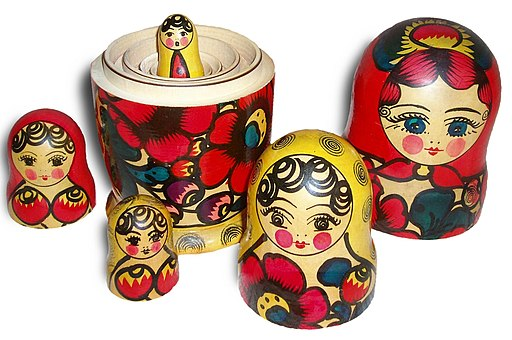
\includegraphics[width=0.3\textwidth]{Figures/dl-nn-ml-ai.jpg}
    \begin{block}{Recap}
        \begin{itemize}
            \item Recap from yesterday
            \item Subset of ML
            \item subset of AI
        \end{itemize}
    \end{block}
\end{frame}
\begin{frame}
    \frametitle{Recap}
    \centering
    \begin{minipage}[c]{0.4\textwidth}
    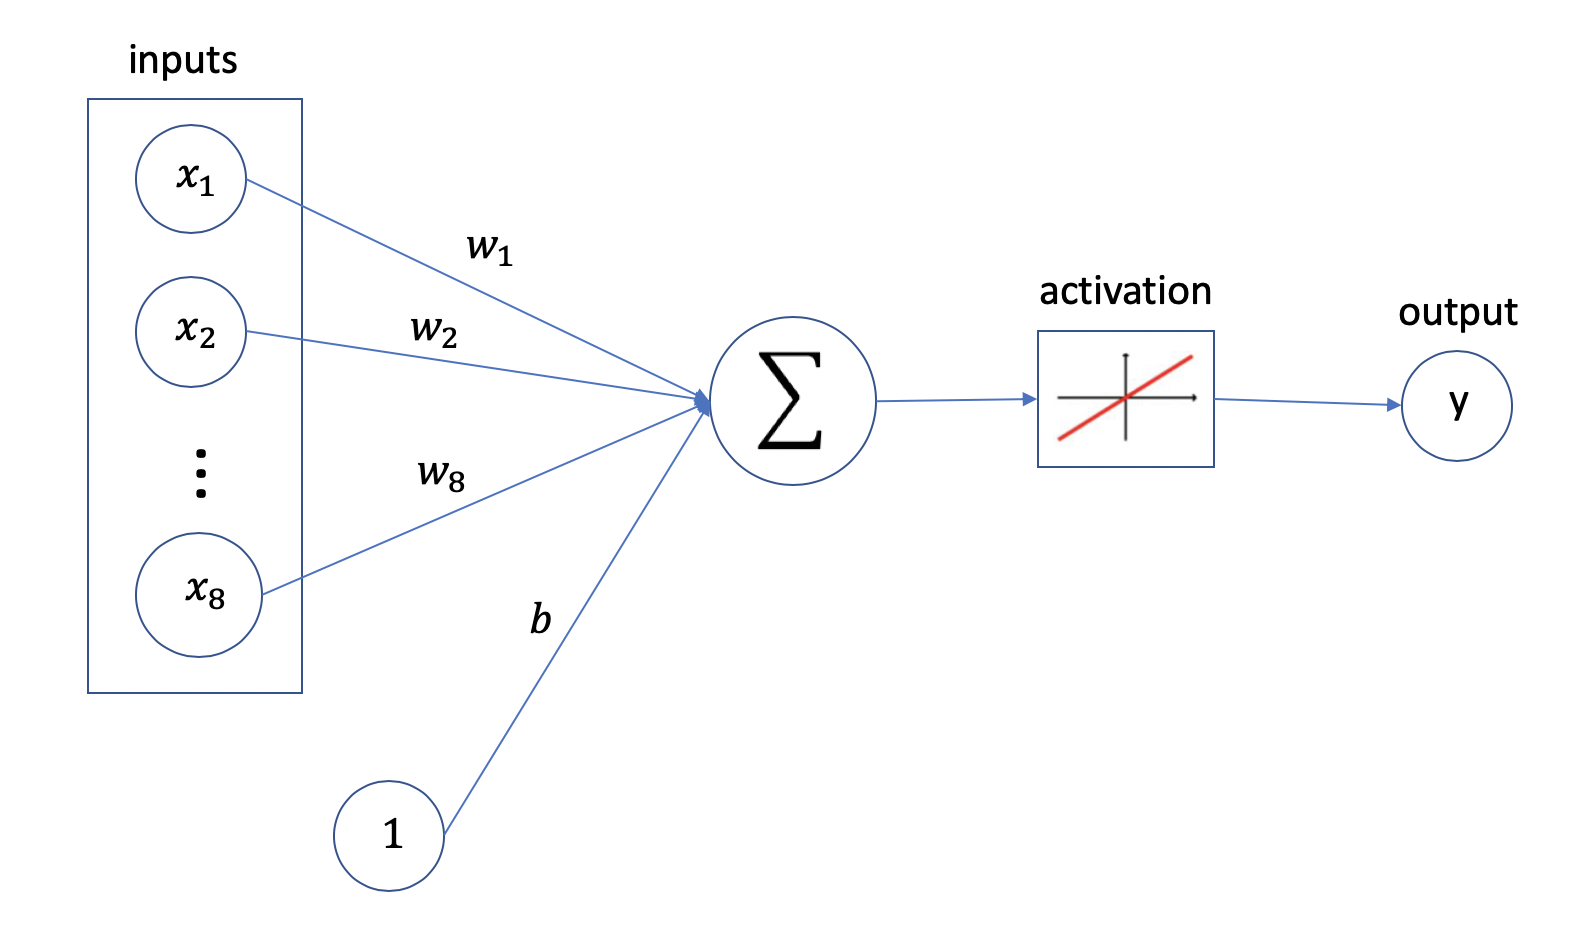
\includegraphics[width=1\textwidth]{Figures/lin-reg.png}
    \end{minipage}
    $MSE=\frac{1}{N}\sum_{i=1}^N({y_i - \hat{y}_i})^2$
    \vspace{-1\baselineskip}
    \begin{block}{How does the network learn?}
        \begin{itemize}
            \item Learns from the difference between expected and true output
            \item Contains many parameter (1e3-1e6)
            \item Calculates the effect of each parameter in the error using back propagation
            \item adjusts the value to minimize the error using gradient descent
        \end{itemize}
    \end{block}
\end{frame}
\begin{frame}
    \frametitle{Recap}
    \begin{block}{Convoluted Learning - Side Note}
        \begin{itemize}
            \item Filter weights and biases learned from data
            \item relies on matrix operations - algeraic math
            \item tech: GPUs are fast. Designed for matrix operations
        \end{itemize}
    \end{block}
\end{frame}
\subsection{Mechanics}
\begin{frame}
    \frametitle{Mechanics}
    \centering
    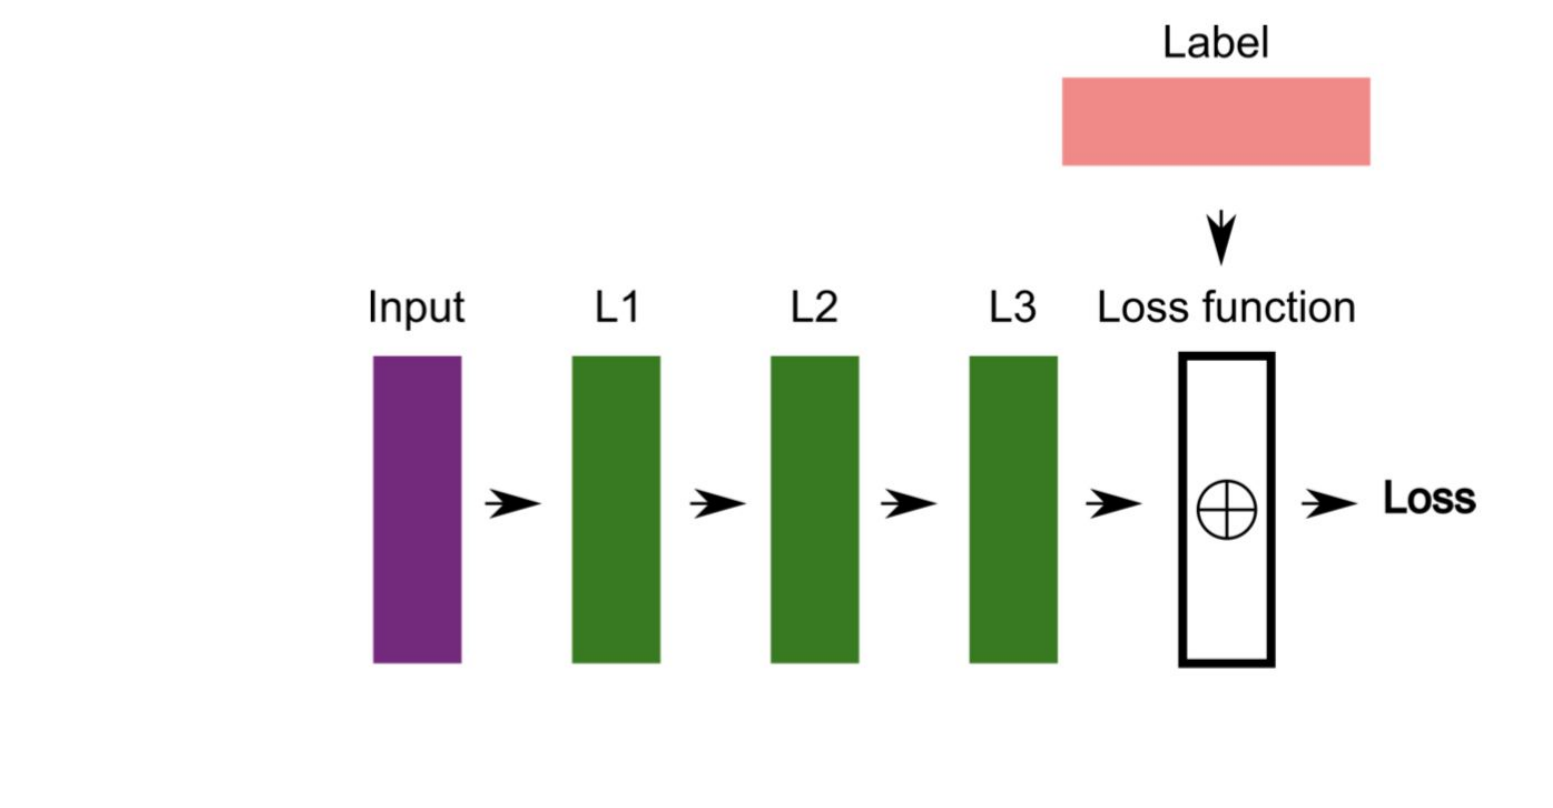
\includegraphics[width=0.6\textwidth]{Figures/forward_pass.png}
    \begin{block}{Forward Pass}
    \end{block}
\end{frame}
\begin{frame}
    \frametitle{Mechanics}
    \centering
    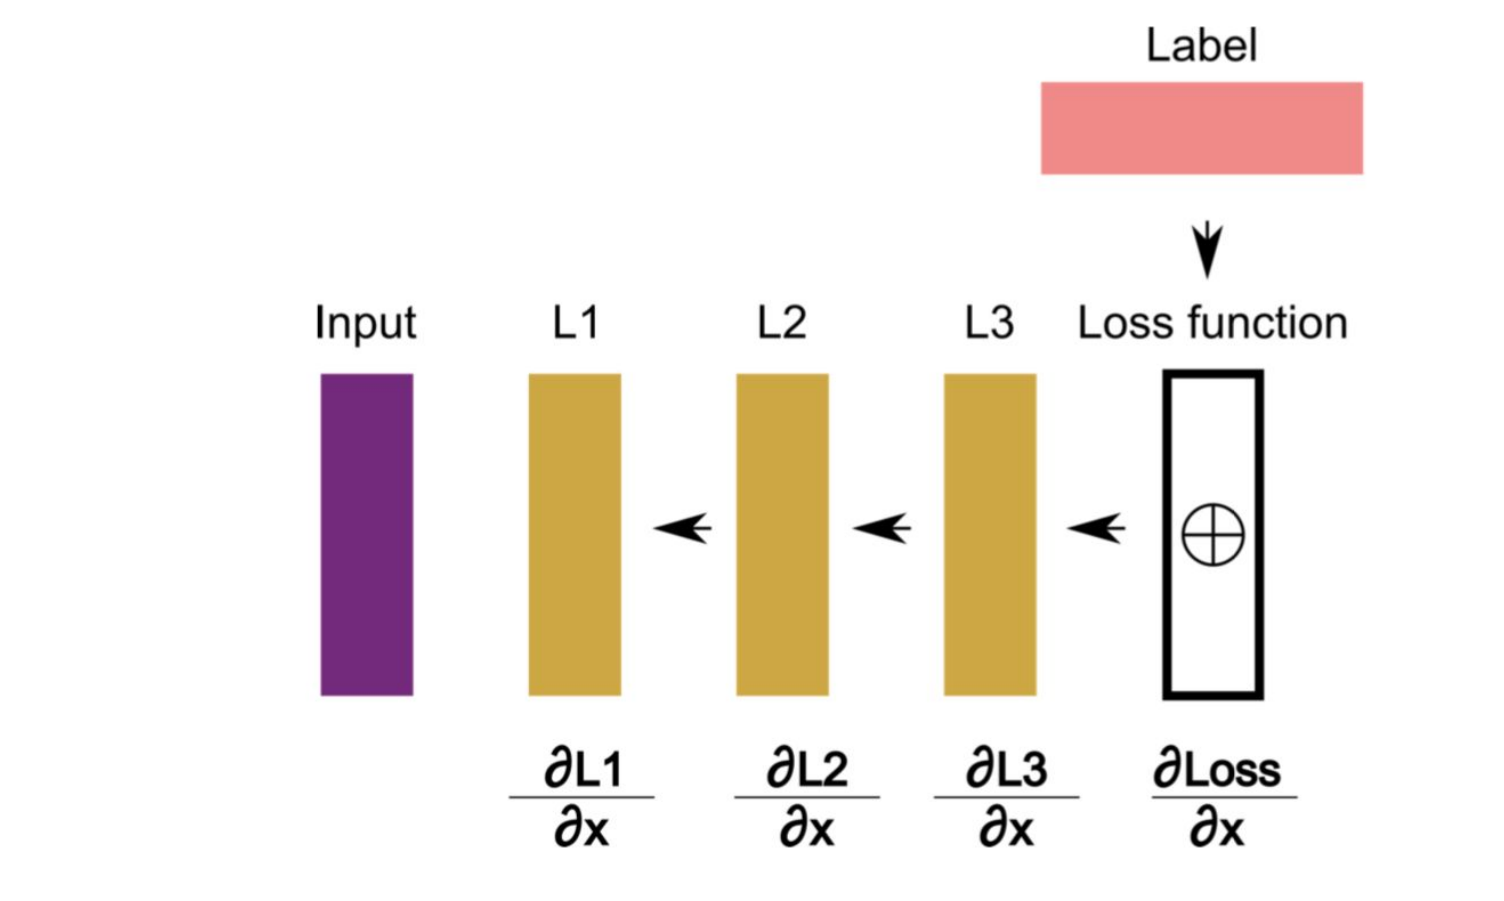
\includegraphics[width=0.6\textwidth]{Figures/back_prop.png}
    \begin{block}{Back Propagation}
    \end{block}
\end{frame}
\begin{frame}
    \frametitle{Mechanics}
    \begin{block}{Gradient Descent}
        \begin{itemize}
            \item Attempts to minimize a function (like a loss) J(x)
            \item For a given Variable x
            \item Is the derivative J'(x) 
            \item Update in the opposite direction of J'(x)
        \end{itemize}
    \end{block}
\end{frame}
\begin{frame}
    \frametitle{Mechanics}
    \centering
    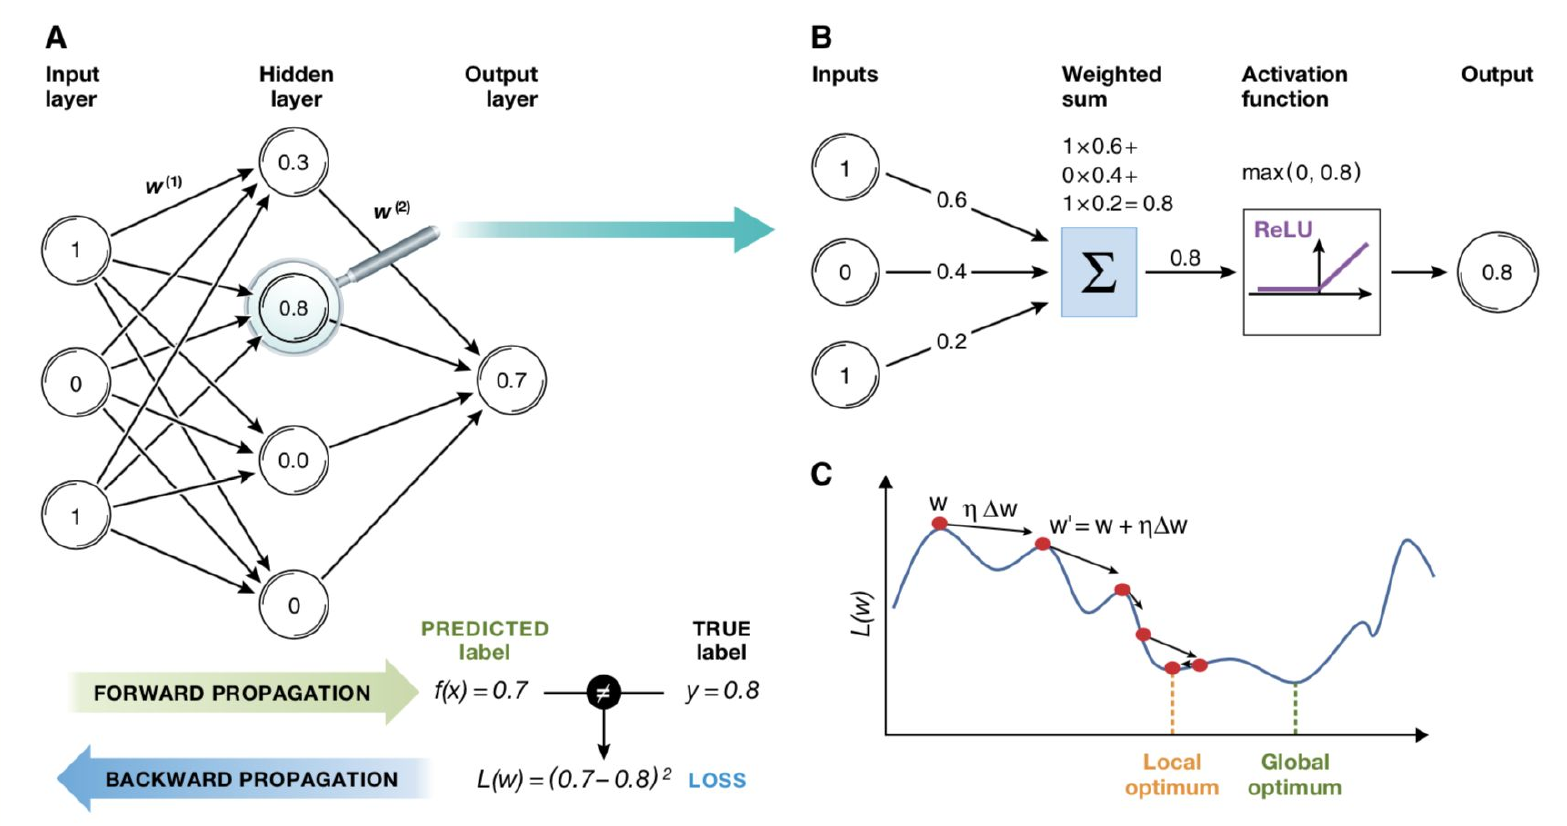
\includegraphics[width=0.6\textwidth]{Figures/overview.png}
    \begin{block}{So! An overview!}
    \end{block}
\end{frame}

\section{Deep Learning - Applications}
\subsection{Overview}
\begin{frame}
    \frametitle{Overview}
    \centering
    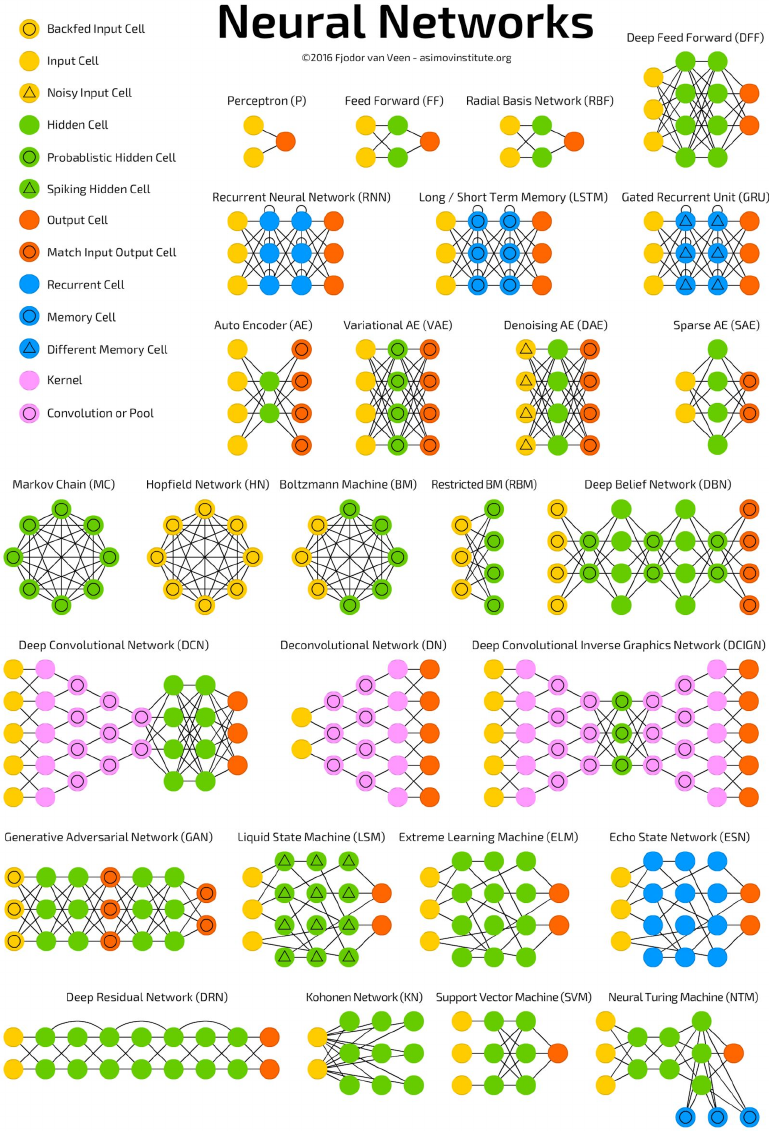
\includegraphics[width=0.1\textwidth]{Figures/variants.png}
    \begin{block}{Multitude of Types:}
        \begin{itemize}
            \item Some require input data and lables
            \item Some automatically learn features from the data
            \item ANNs ideal for vectors (i.e sequences)
            \item CNNs ideal for matrixes (i. e images)
        \end{itemize}
    \end{block}
\end{frame}
\begin{frame}
    \frametitle{Overview}
    \begin{block}{Multitude of Types:}
        \begin{itemize}
            \item Sequence Analysis
            \item Image Analysis
            \item Object Tracking
            \item Segmentation
        \end{itemize}
    \end{block}
\end{frame}

\subsection{Image Analysis}
\begin{frame}
    \frametitle{Image Analysis}
    \centering
    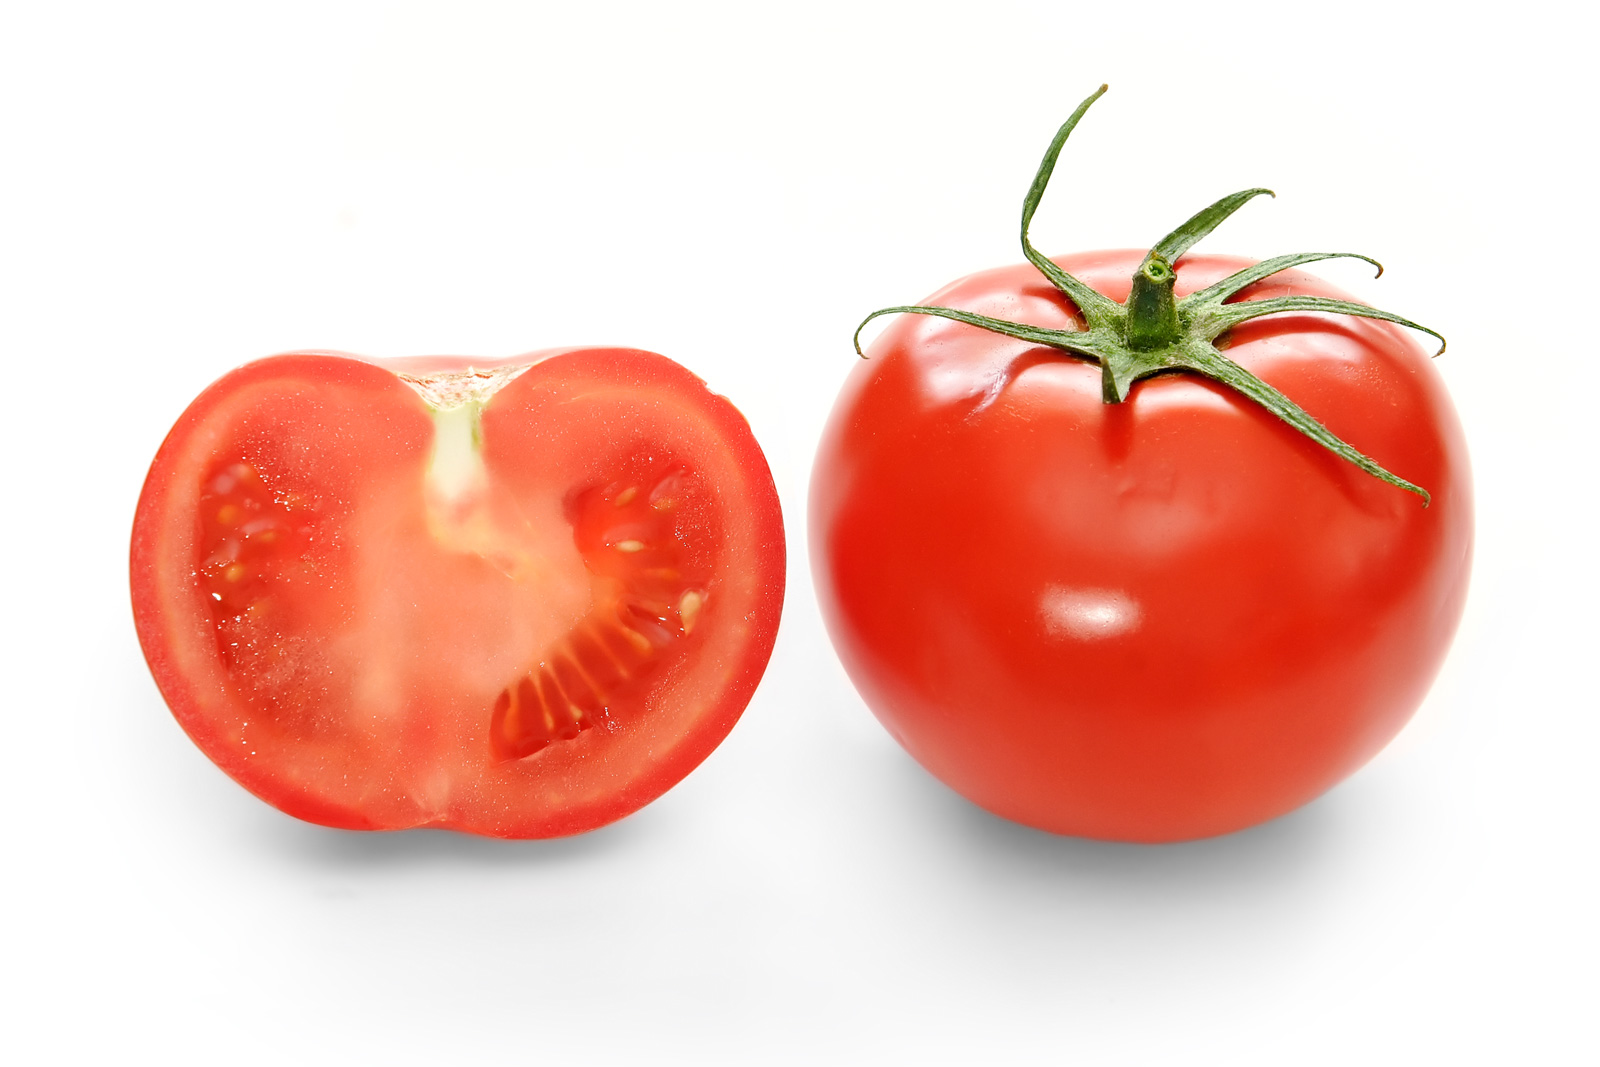
\includegraphics[width=0.3\textwidth]{Figures/small_tomato.jpg}
    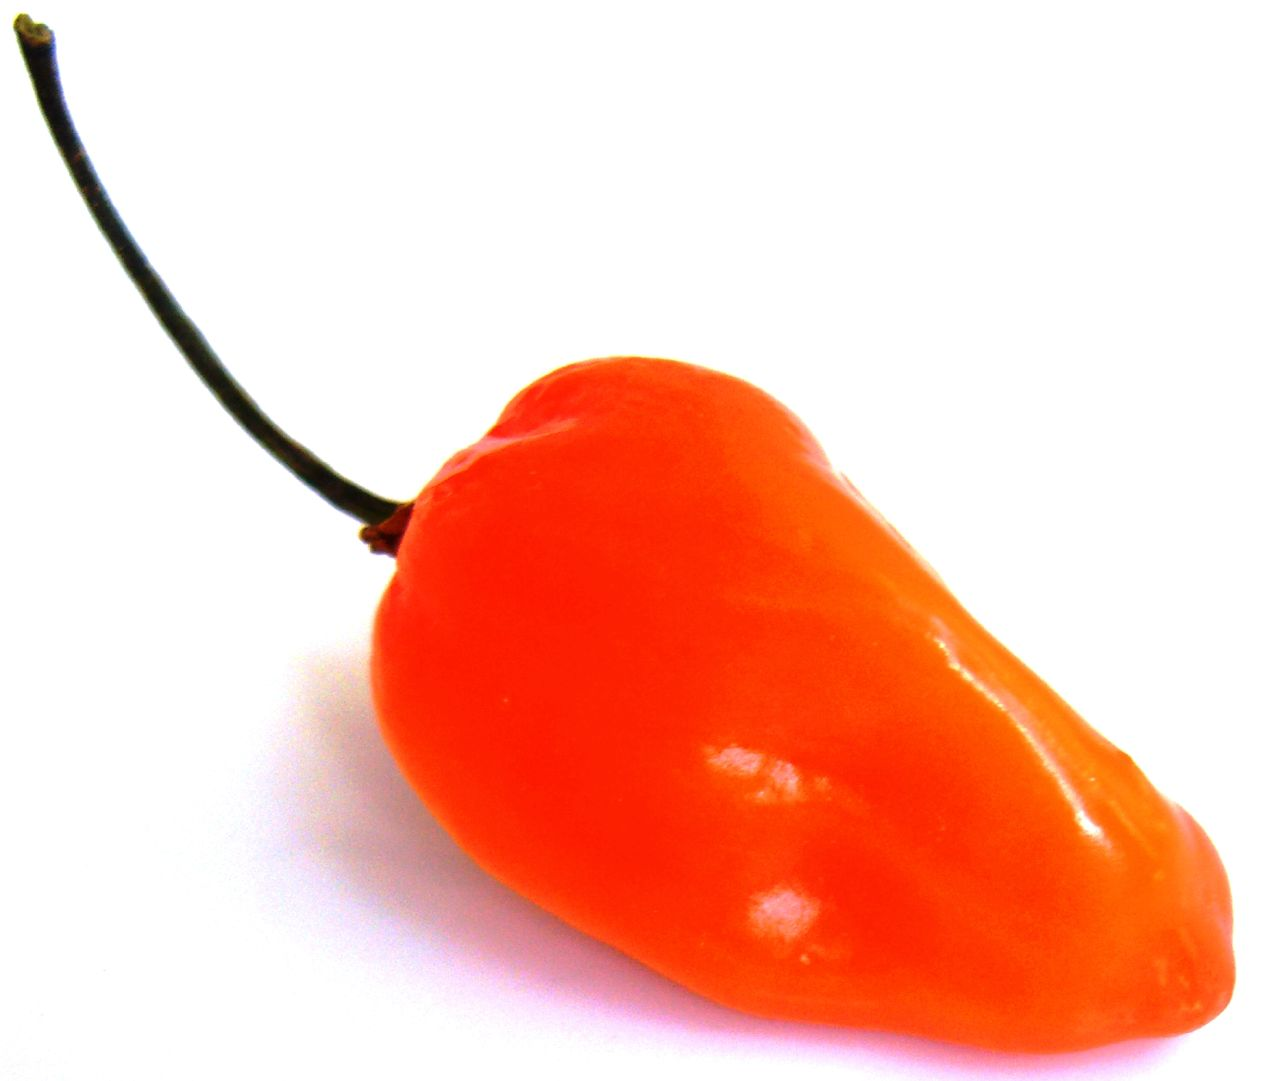
\includegraphics[width=0.2\textwidth]{Figures/chili.jpg}
    \begin{block}{Classification models}
        \begin{itemize}
            \item Classify data into categories
            \item Is this a chili-fruit or a tomato?
            \item Is this mushroom toxic?
            \item Image recognition is Hard
        \end{itemize}
    \end{block}
\end{frame}
\begin{frame}
    \frametitle{Image Analysis}
    \centering
    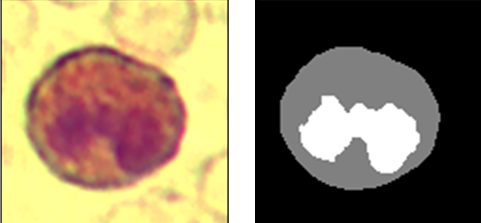
\includegraphics[width=0.4\textwidth]{Figures/eosinophile.png}
    \vspace{-0.9\baselineskip}
    \begin{block}{problems?}
        \begin{itemize}
            \item Segment data into smaller yet relevant pieces of data
            \item is that 10 mononucleated cells, or 5 multinucleated cells in the image?
        \end{itemize}
    \end{block}
\end{frame}
\begin{frame}
    \frametitle{Image Analysis}
    \begin{block}{Problems.}
        \begin{itemize}
            \item Multiple Challenges
            \item Lets look at stanford cats to exemplify
            \item (since apparently we like cats in this group...)
        \end{itemize}
    \end{block}
\end{frame}

\begin{frame}
    \frametitle{Image Analysis}
    \centering
    \vspace{-1.2\baselineskip}
    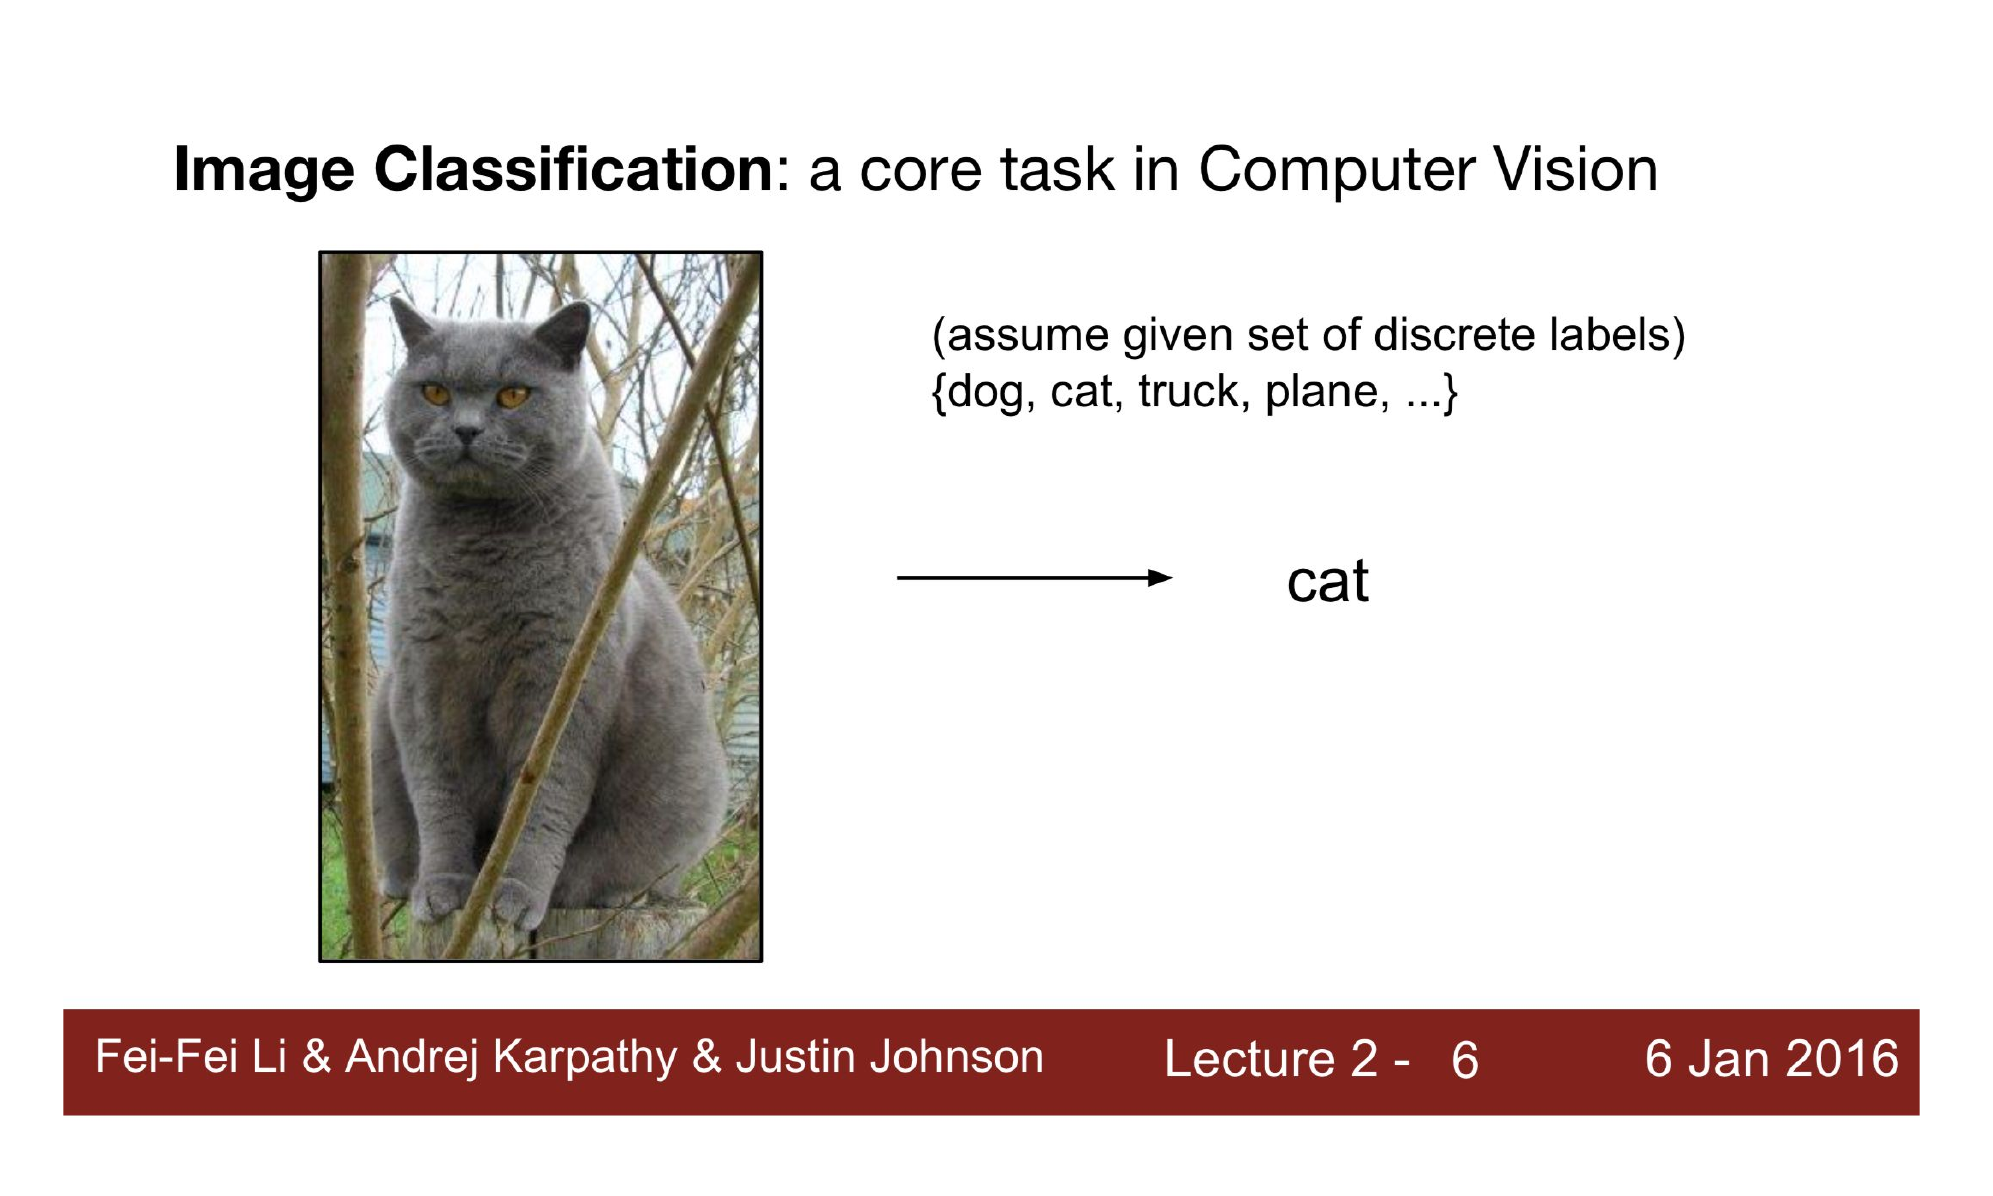
\includegraphics[width=0.7\textwidth]{Figures/stn1.png}
\end{frame}
\begin{frame}
    \frametitle{Image Analysis}
    \centering
    \vspace{-1.2\baselineskip}
    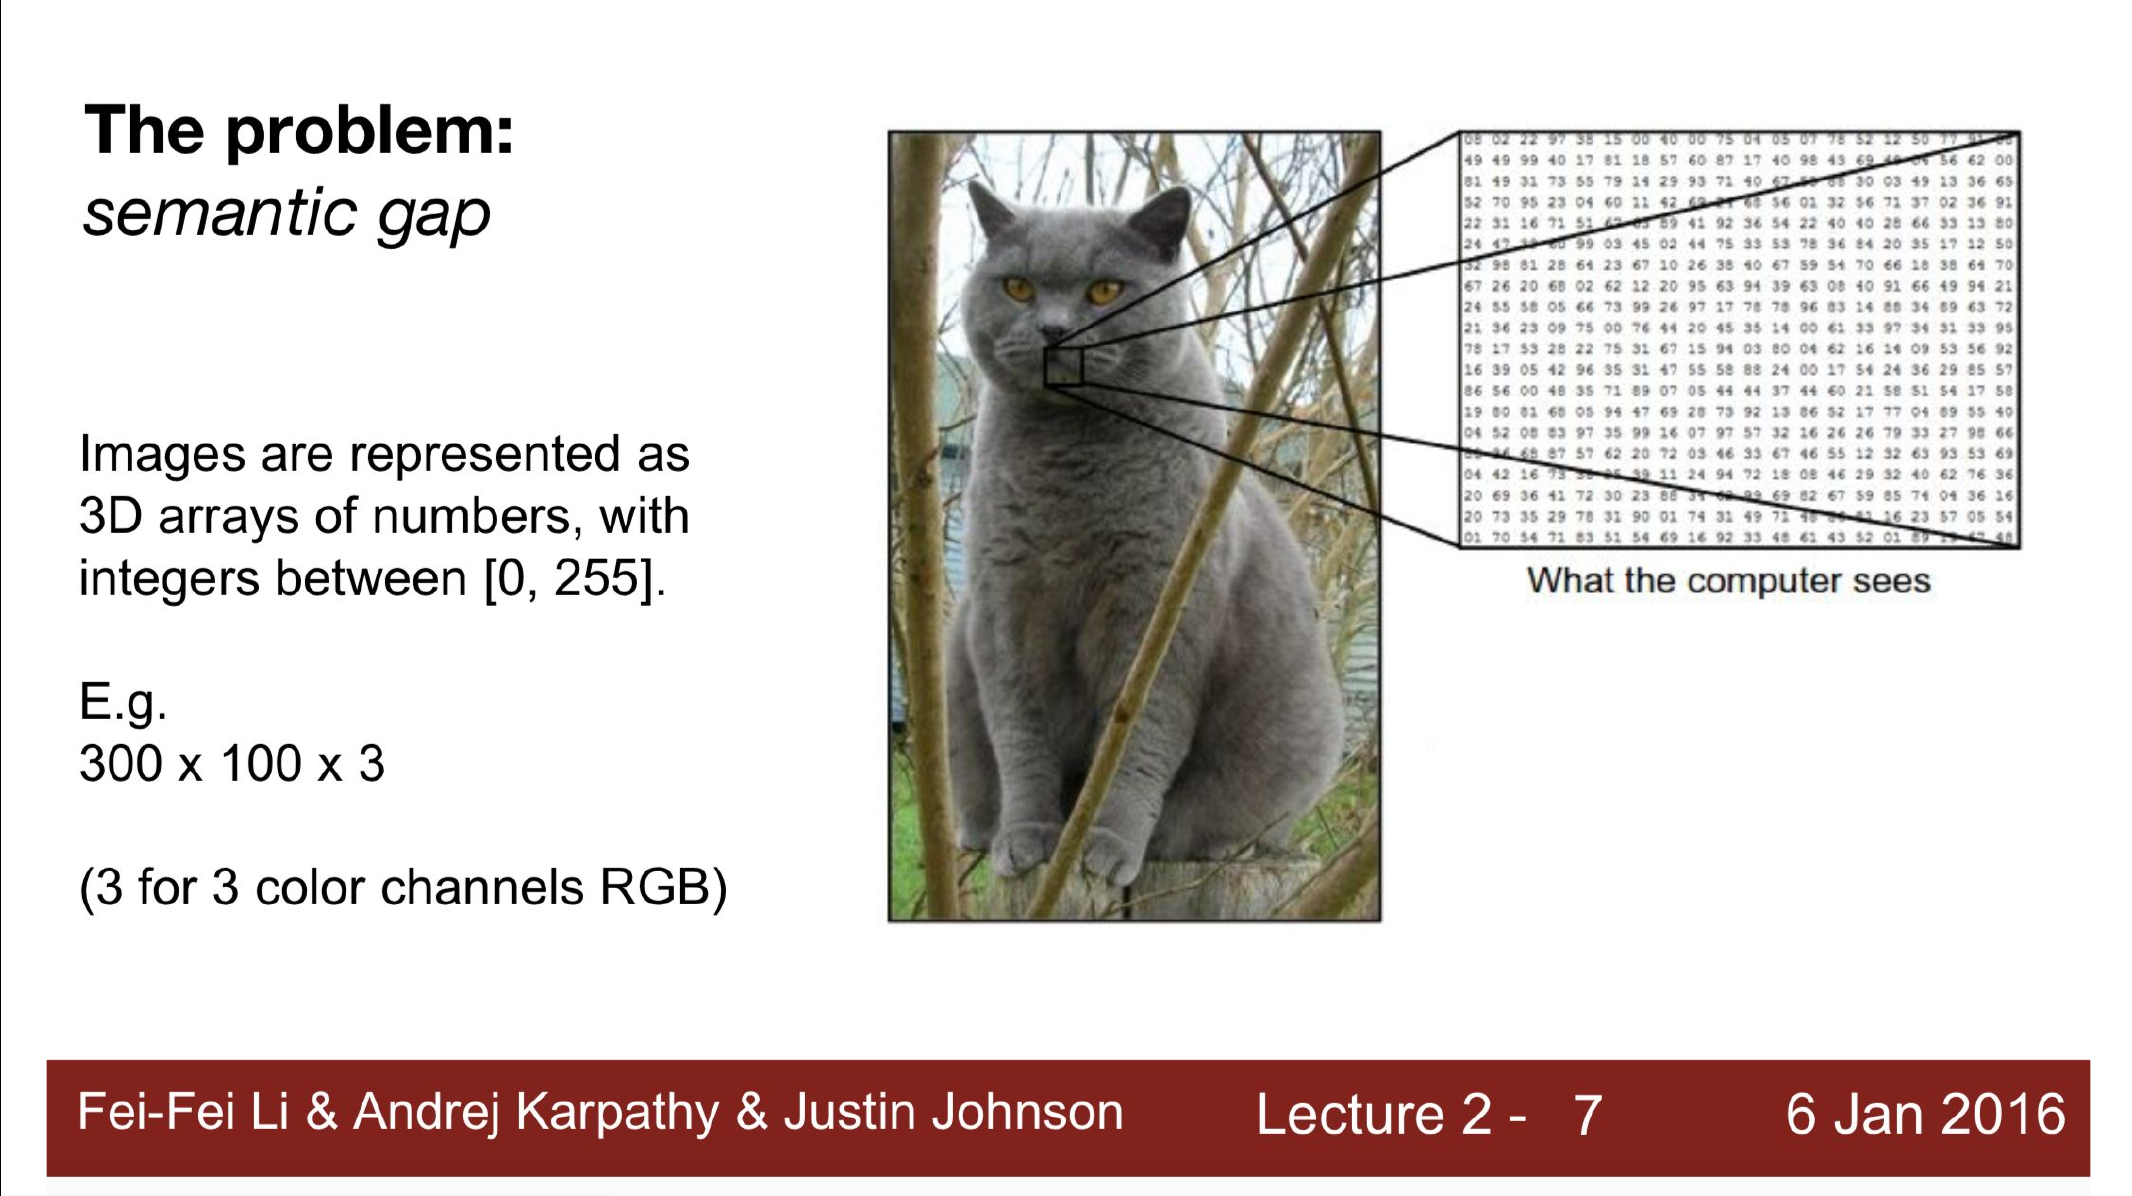
\includegraphics[width=0.7\textwidth]{Figures/stn2.png}
\end{frame}
\begin{frame}
    \frametitle{Image Analysis}
    \centering
    \vspace{-1.2\baselineskip}
    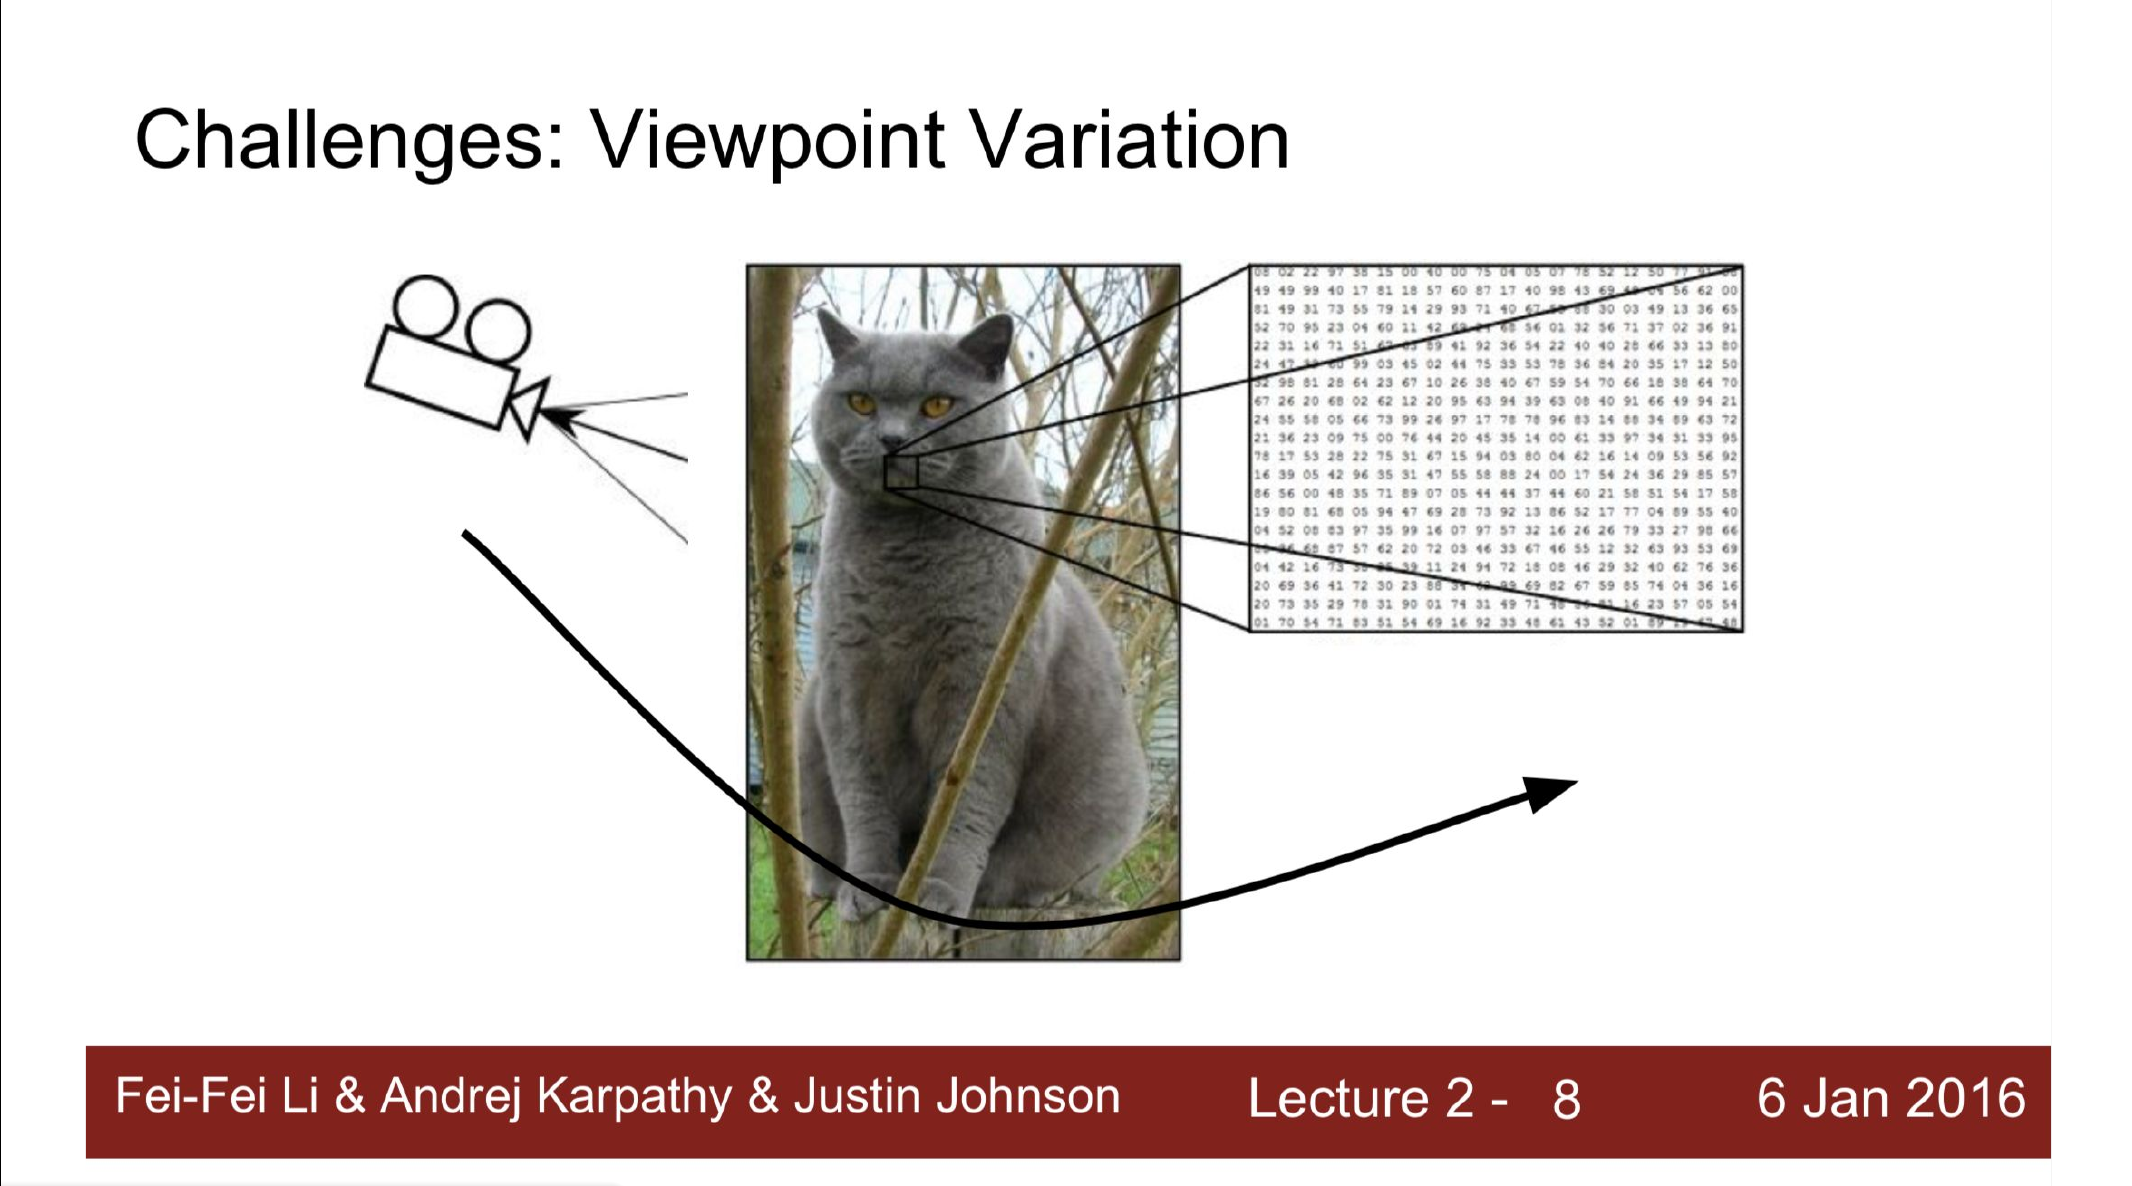
\includegraphics[width=0.7\textwidth]{Figures/stn3.png}
\end{frame}
\begin{frame}
    \frametitle{Image Analysis}
    \centering
    \vspace{-1.2\baselineskip}
    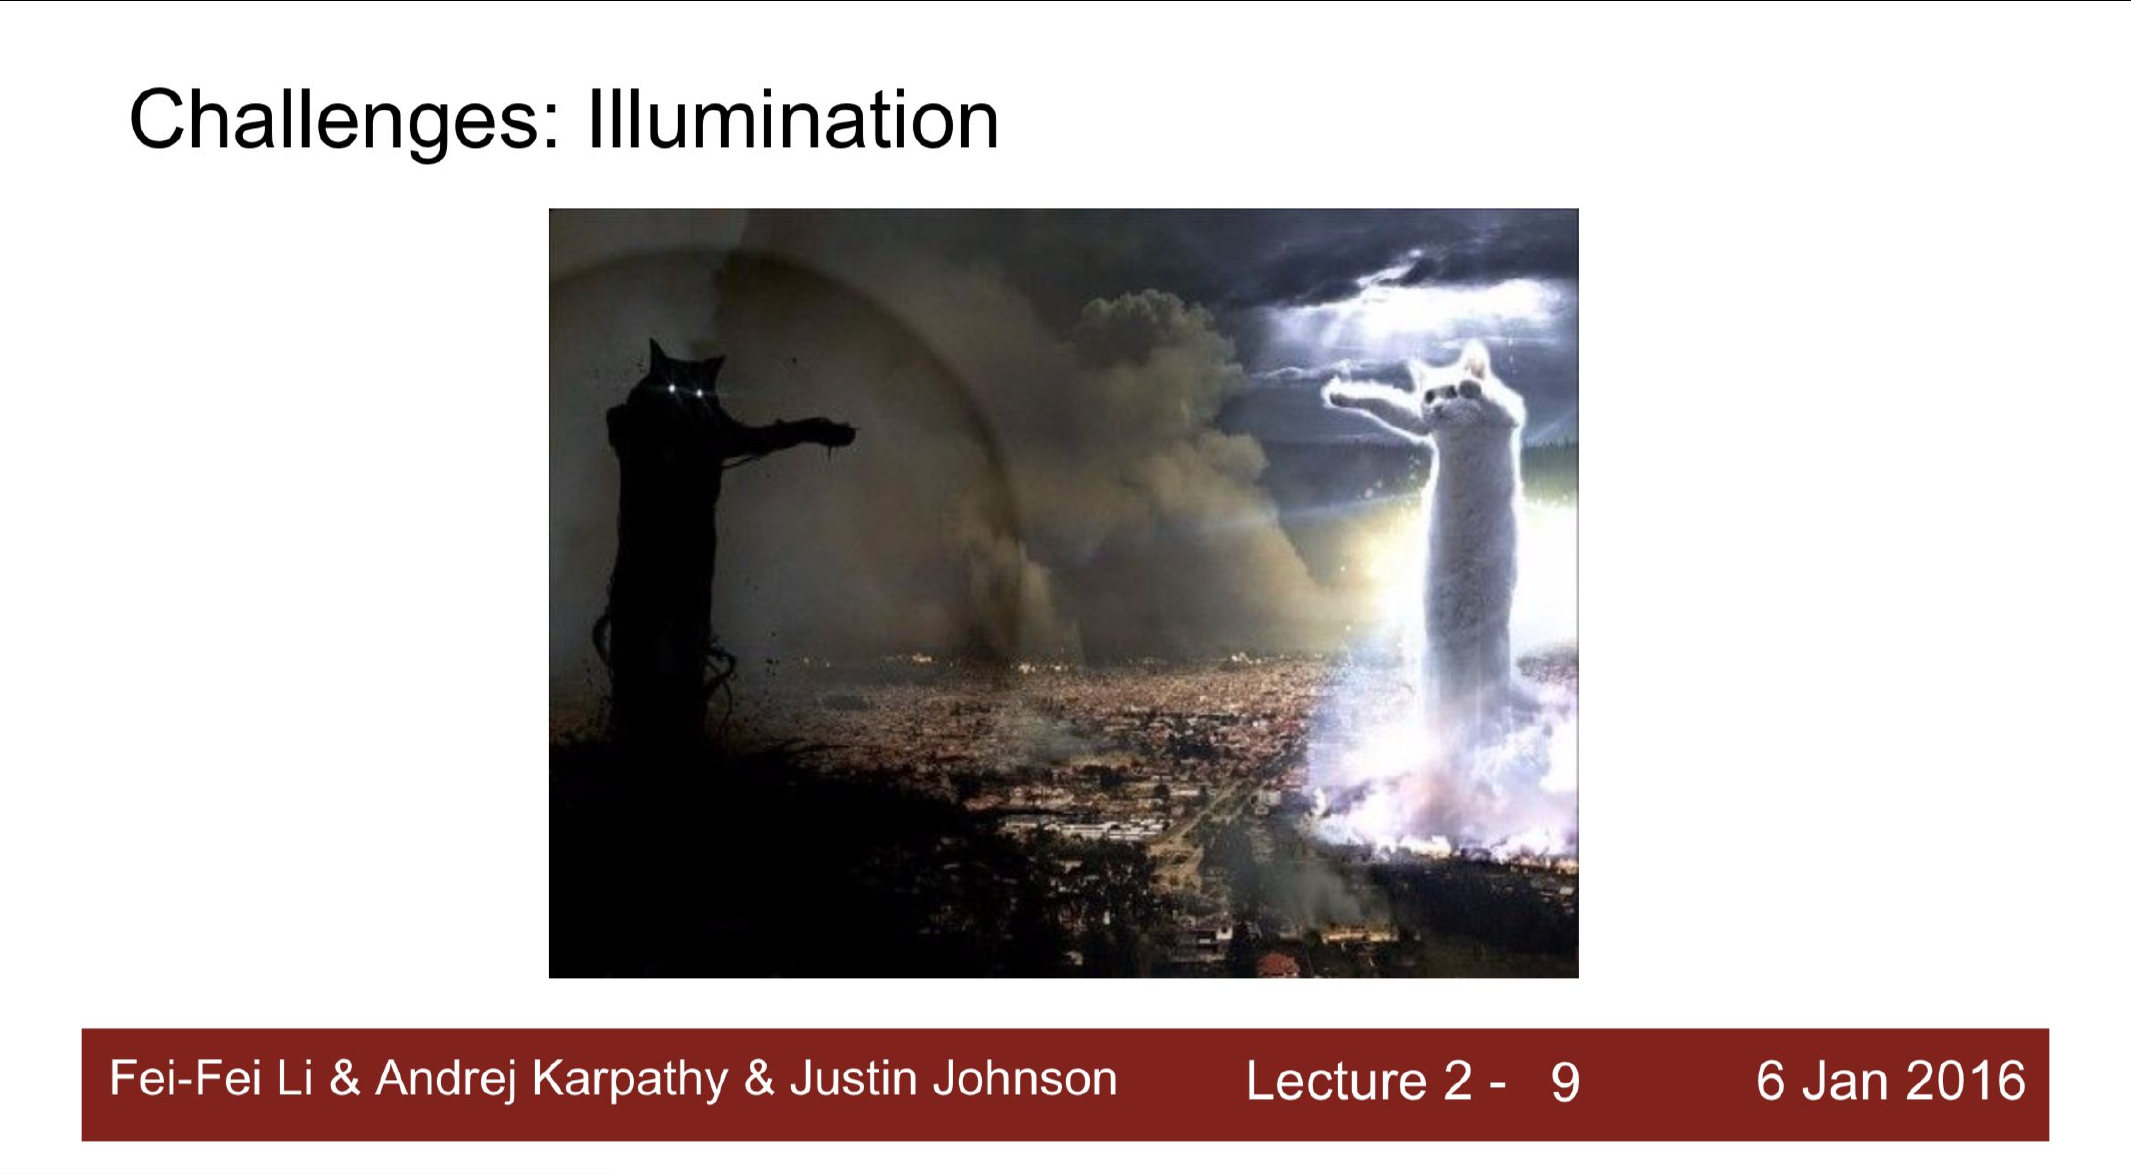
\includegraphics[width=0.7\textwidth]{Figures/stn4.png}
\end{frame}
\begin{frame}
    \frametitle{Image Analysis}
    \centering
    \vspace{-1.2\baselineskip}
    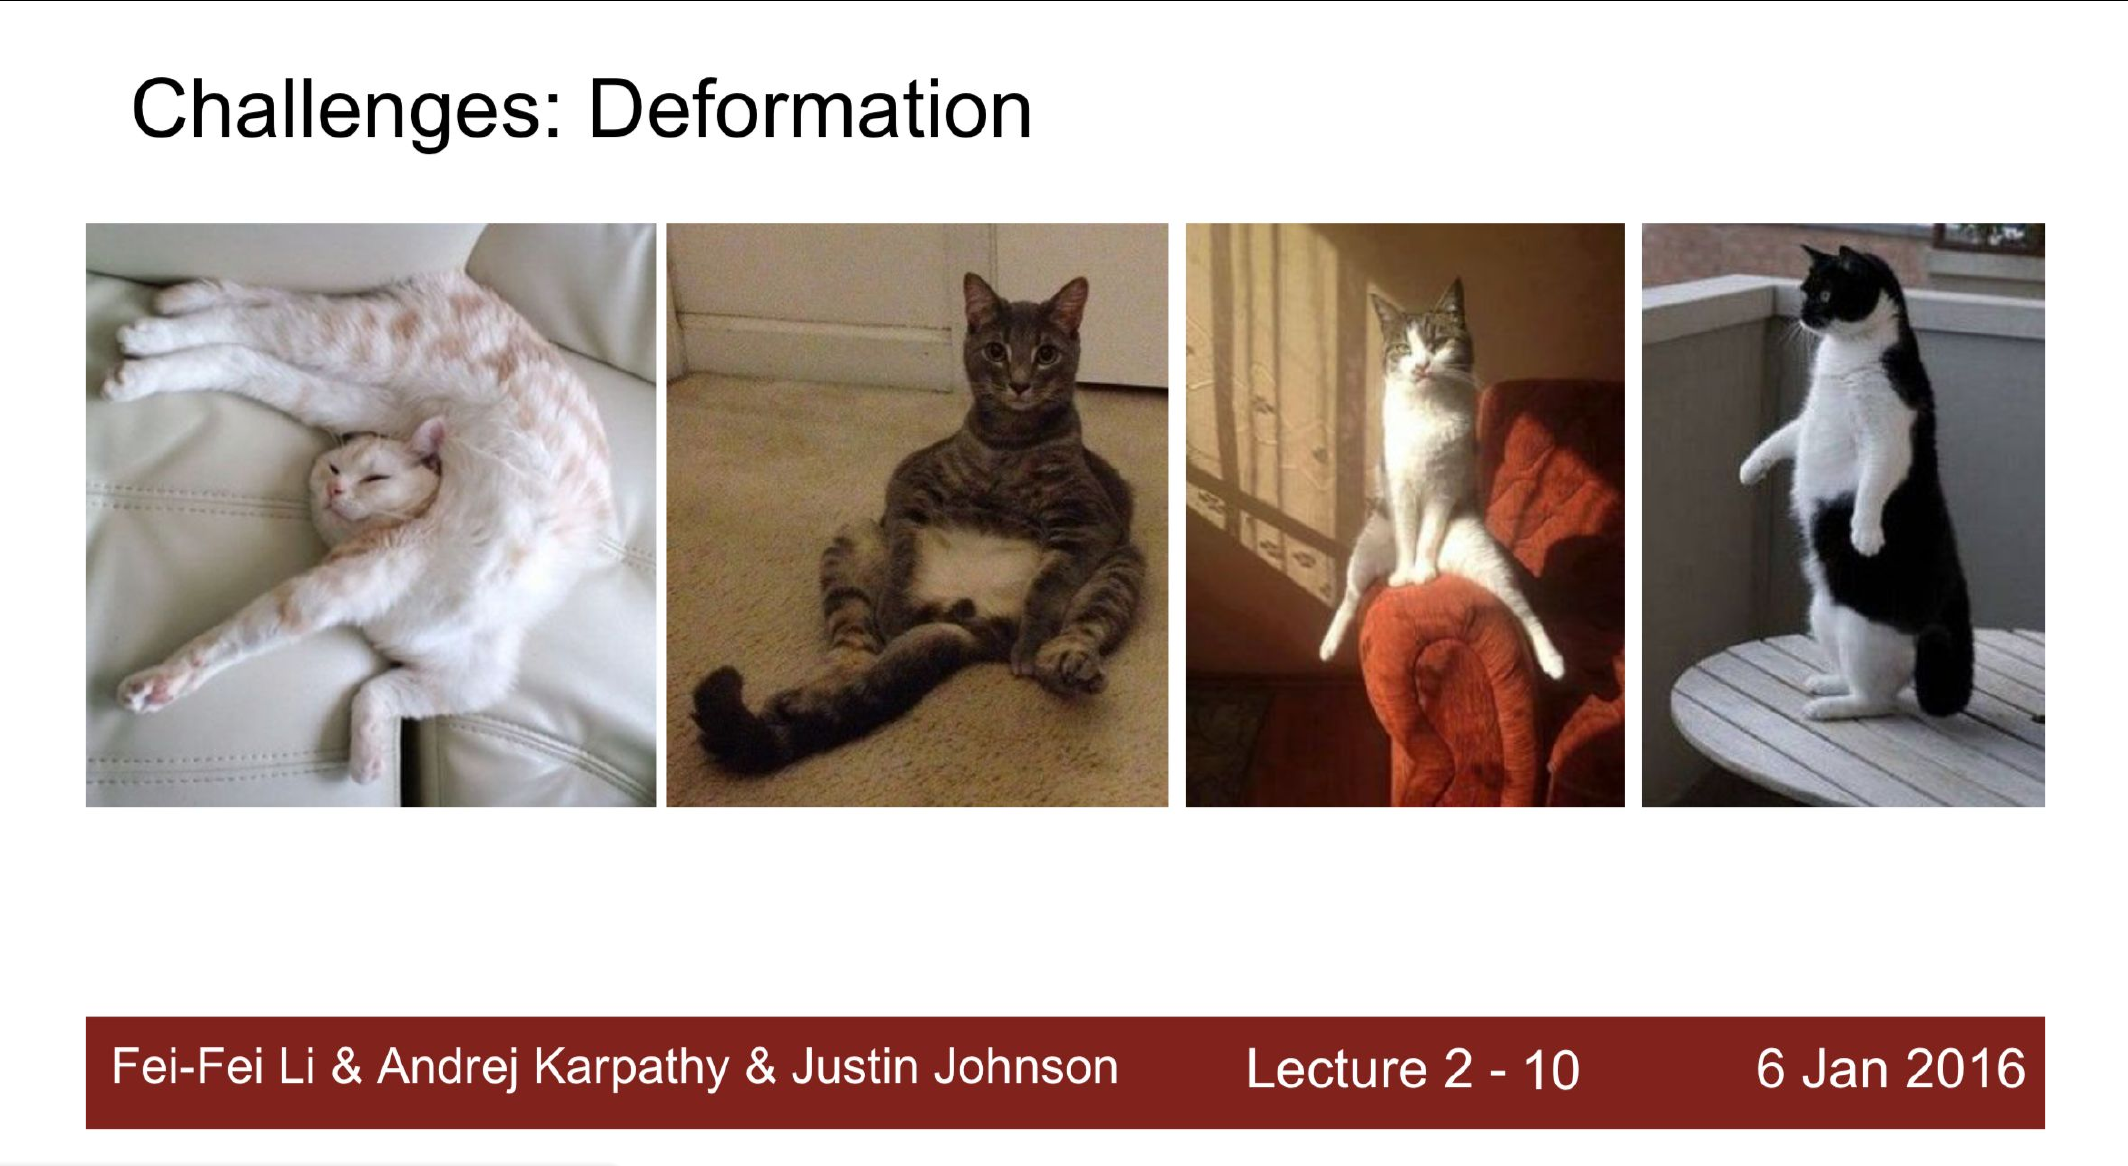
\includegraphics[width=0.7\textwidth]{Figures/stn5.png}
\end{frame}
\begin{frame}
    \frametitle{Image Analysis}
    \centering
    \vspace{-1.2\baselineskip}
    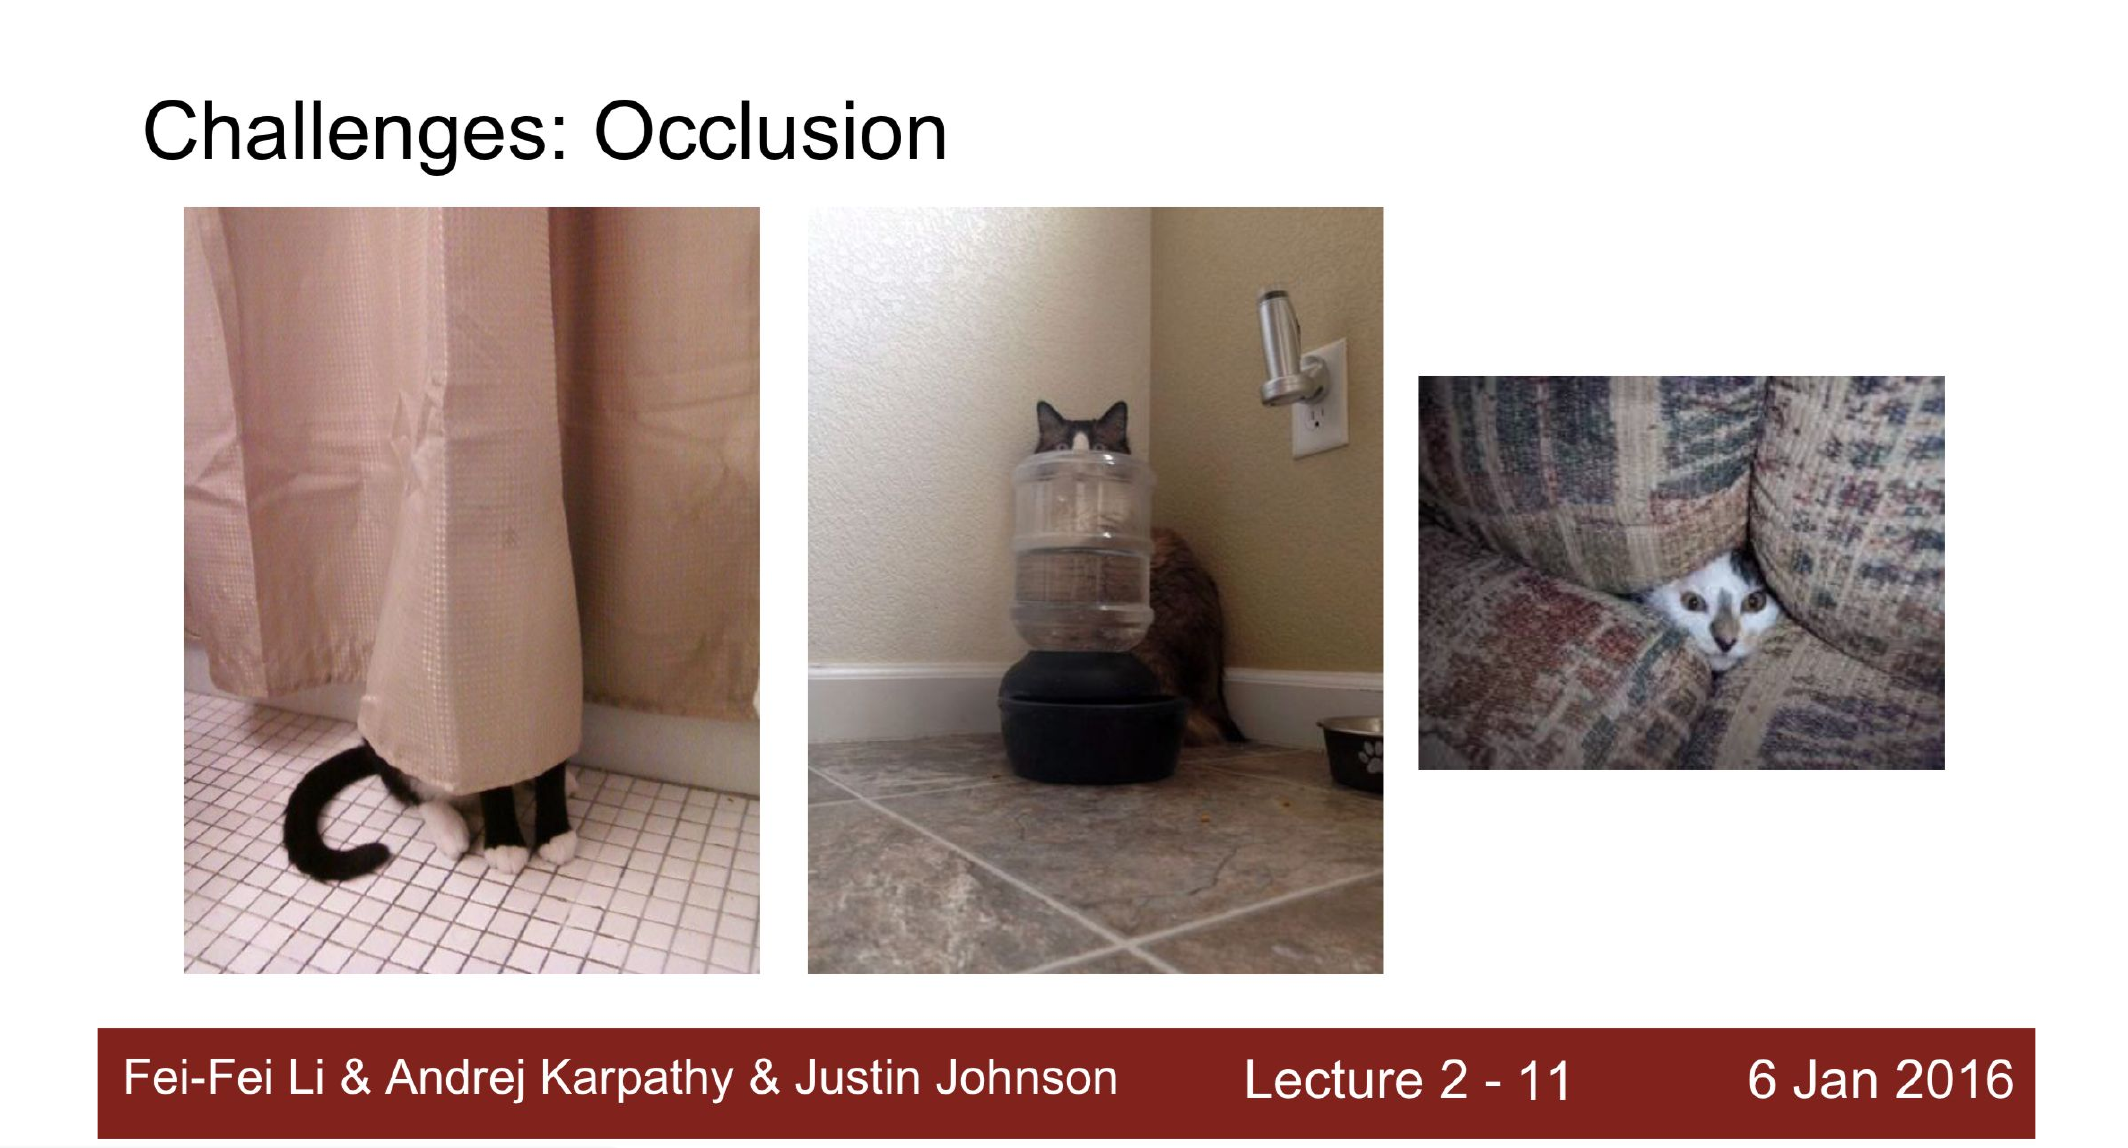
\includegraphics[width=0.7\textwidth]{Figures/stn6.png}
\end{frame}
\begin{frame}
    \frametitle{Image Analysis}
    \centering
    \vspace{-1.2\baselineskip}
    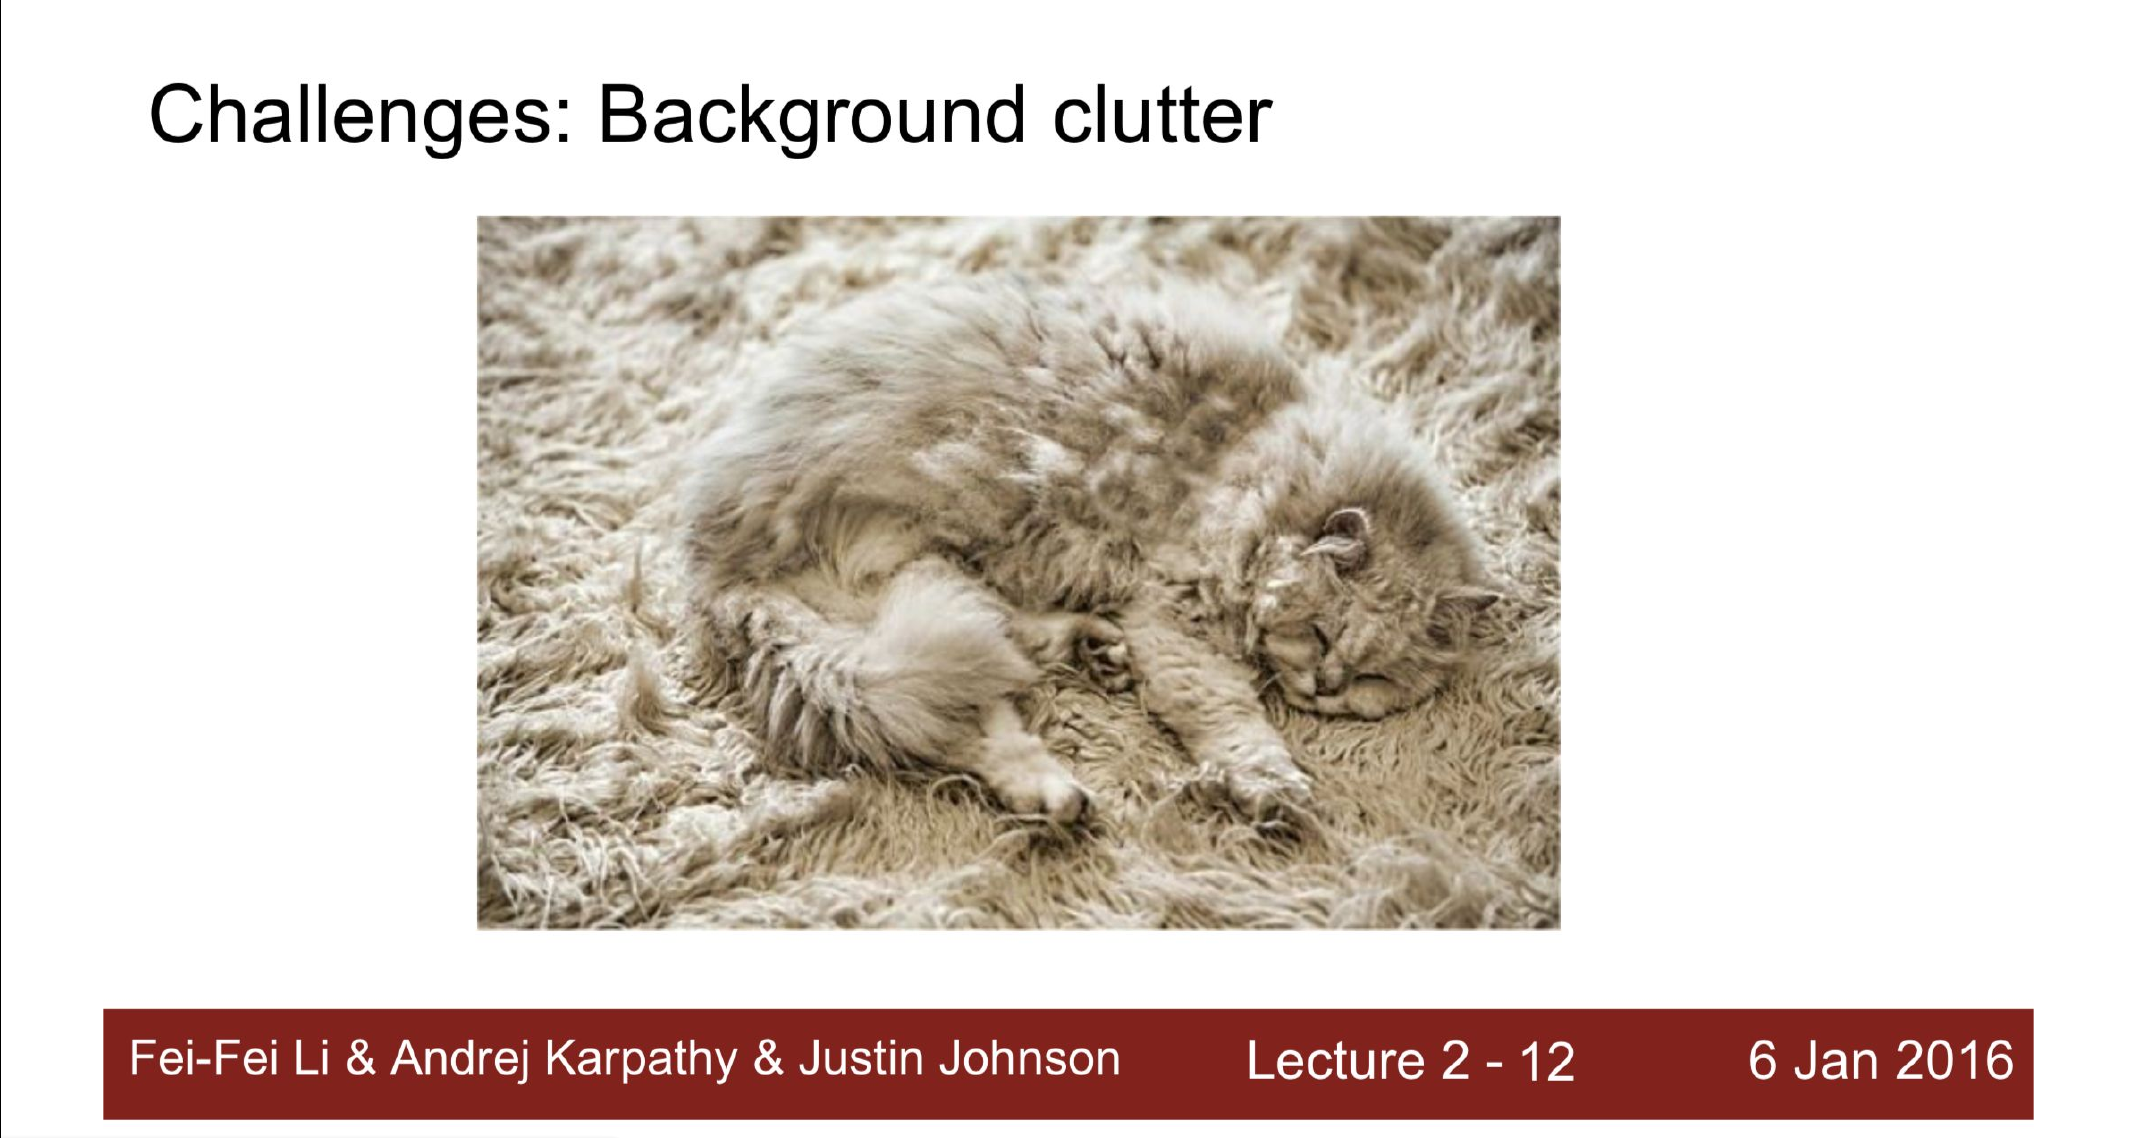
\includegraphics[width=0.7\textwidth]{Figures/stn7.png}
\end{frame}
\begin{frame}
    \frametitle{Image Analysis}
    \centering
    \vspace{-1.2\baselineskip}
    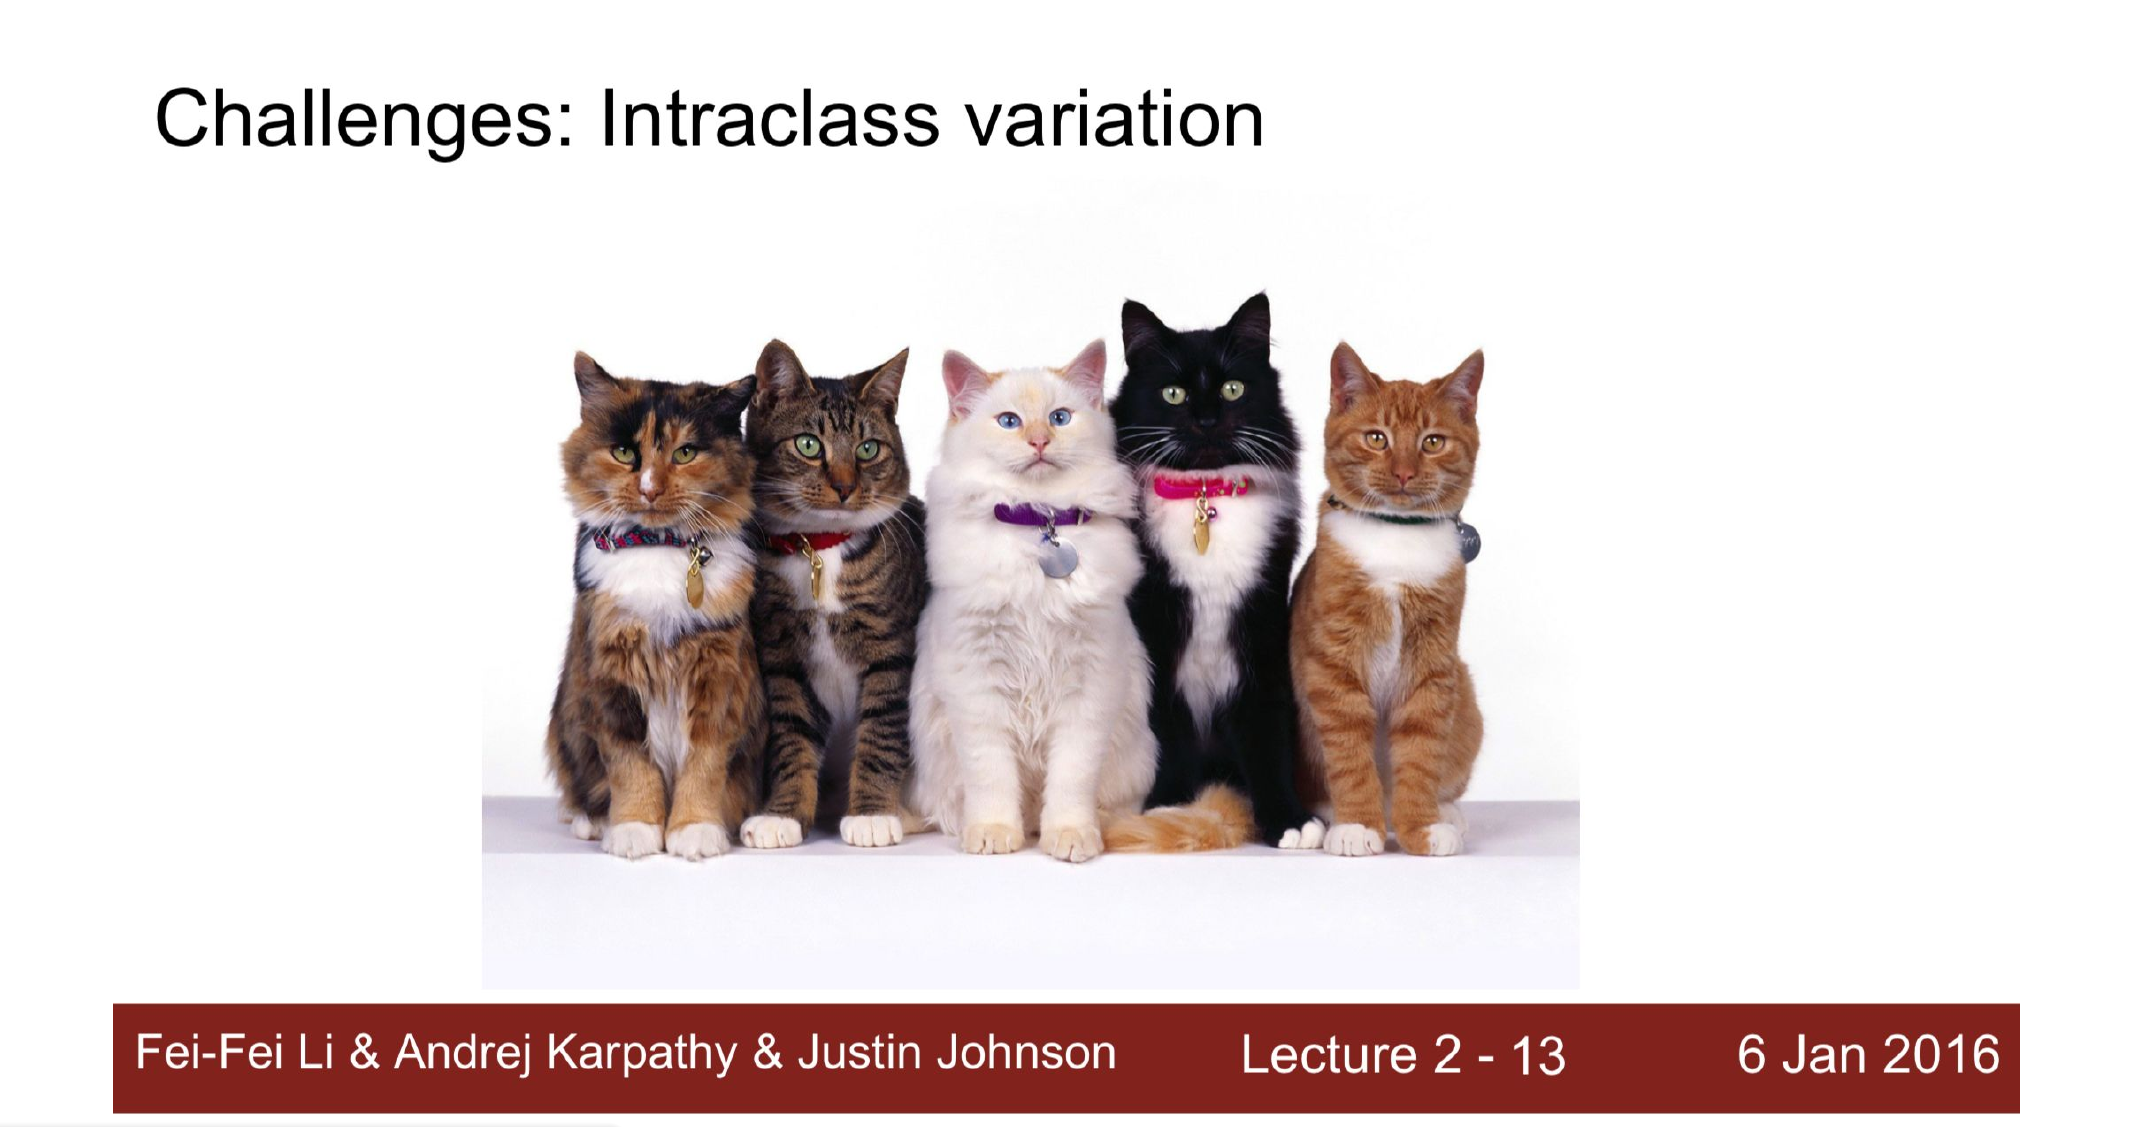
\includegraphics[width=0.7\textwidth]{Figures/stn8.png}
\end{frame}
\begin{frame}
    \frametitle{Image Analysis}
    \begin{block}{Labeled}
        \begin{itemize}
            \item Sets of images and label for training
            \item model learns to distinguish between extant lables
            \item "cat" "dog" "fox" "not-cat" etc       
        \end{itemize}
    \end{block}
\end{frame}
\begin{frame}
    \frametitle{Image Analysis}
    \begin{block}{unlabeled}
        \begin{itemize}
            \item "Unsupervised" "Self-supervised"
            \item Very similar though.
            \item Learns from most sigificant features      
        \end{itemize}
    \end{block}
\end{frame}



\subsection{The Boilerplate}
\begin{frame}
    \frametitle{The Boilerplate}
    \centering
    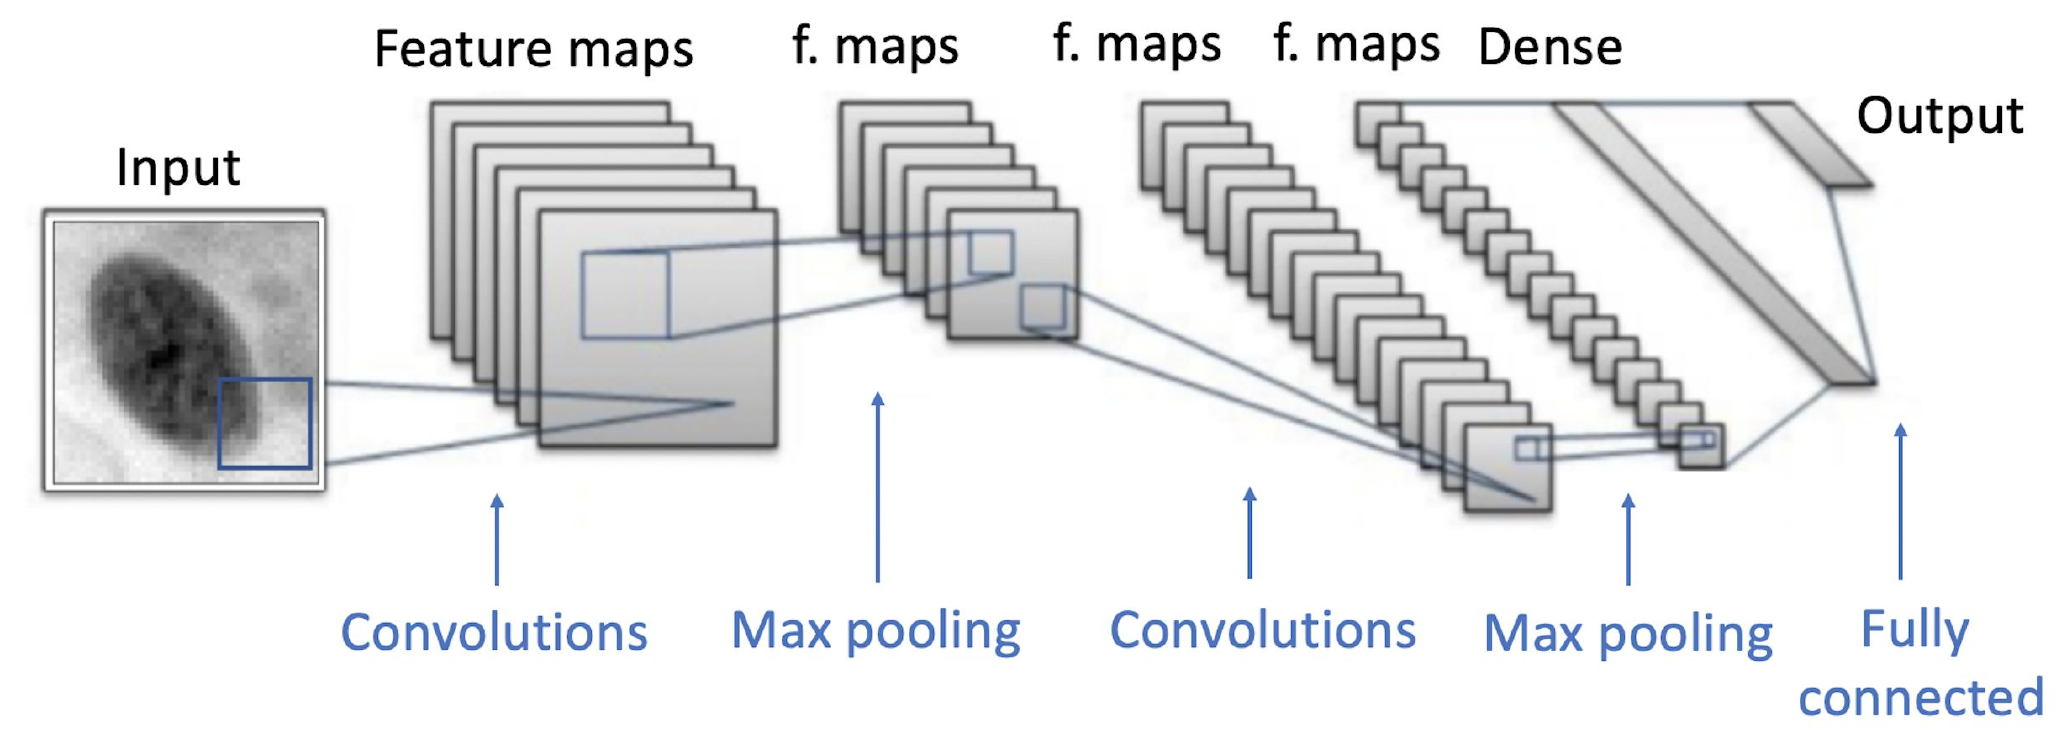
\includegraphics[width=0.6\textwidth]{Figures/basicCNN.png}
    \begin{block}{a CNN}
        \begin{itemize}
            \item each layer detects features        
        \end{itemize}
    \end{block}
\end{frame}
\begin{frame}
    \frametitle{The Boilerplate}
    \centering
    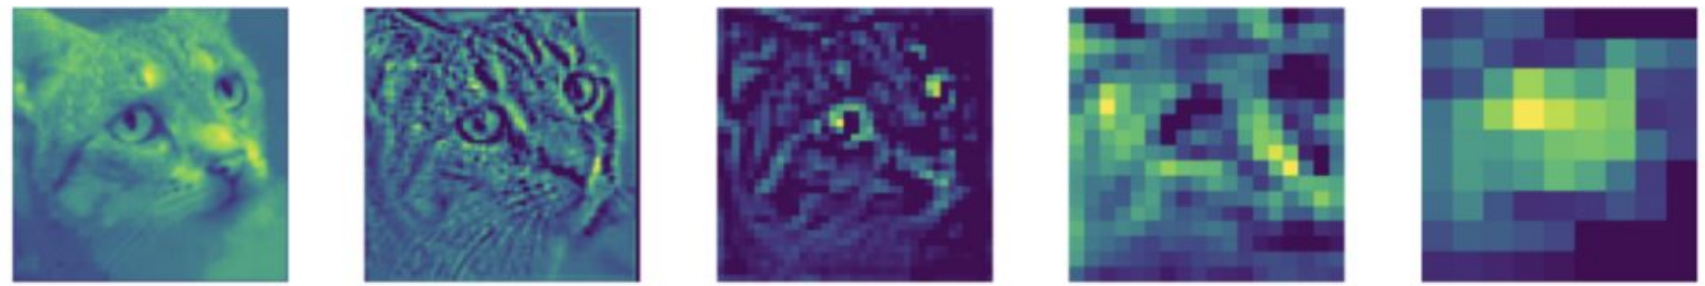
\includegraphics[width=0.7\textwidth]{Figures/catfeat.png}
    \begin{block}{what the network learns}
        \begin{itemize}
            \item each layer detects features        
        \end{itemize}
    \end{block}
\end{frame}
\begin{frame}
    \frametitle{The Boilerplate}
    \centering
    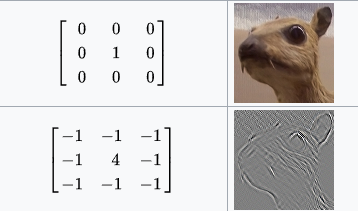
\includegraphics[width=0.45\textwidth]{Figures/kernel.png}
    \vspace{-1\baselineskip}
    \begin{block}{Convoluted Operations}
        \begin{itemize}
            \item Based on Digital Image Analysis methods
            \item As implied, works best on image data
            \item works well on any 2D matrix data
        \end{itemize}
    \end{block}
\end{frame}
\begin{frame}
    \frametitle{The Boilerplate}
    \centering
    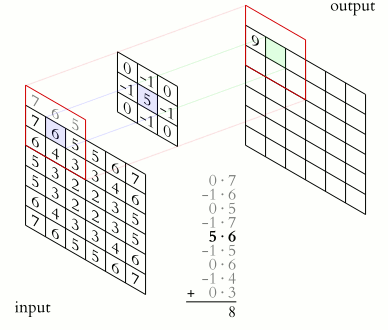
\includegraphics[width=0.28\textwidth]{Figures/kernel2.png}
    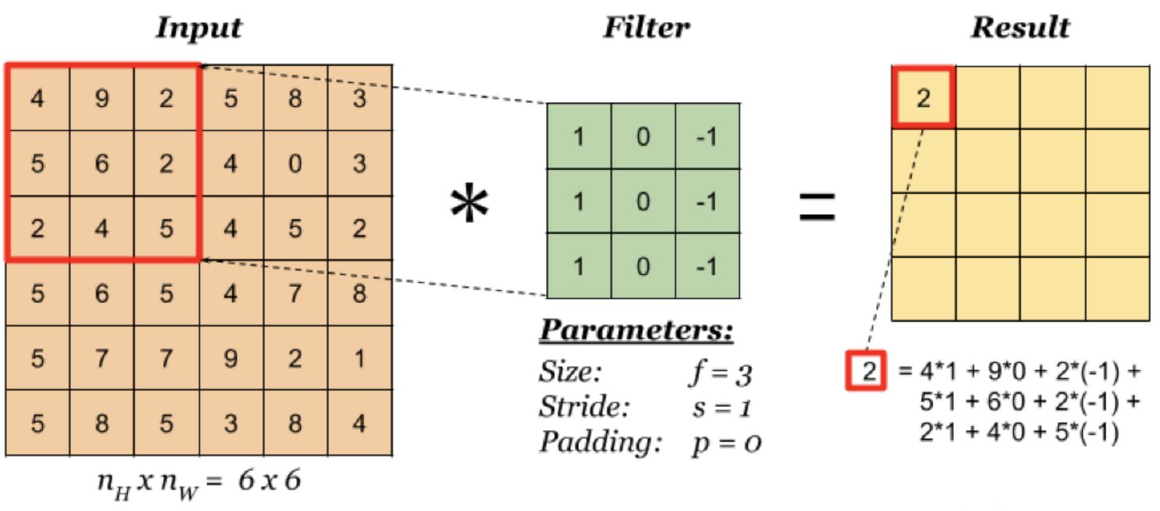
\includegraphics[width=0.45\textwidth]{Figures/kernel3.png}
    \vspace{-1\baselineskip}
    \begin{block}{Convoluted Operations}
        \begin{itemize}
            \item Roving Kernel over the data
            \item Each Kernel learns a weight
            \item Builds up "new" tensor as input for next layer
            \item Error is backpropagated through the layer, like before   
        \end{itemize}    
    \end{block}
\end{frame}
\begin{frame}
    \frametitle{The Boilerplate}
    \centering
    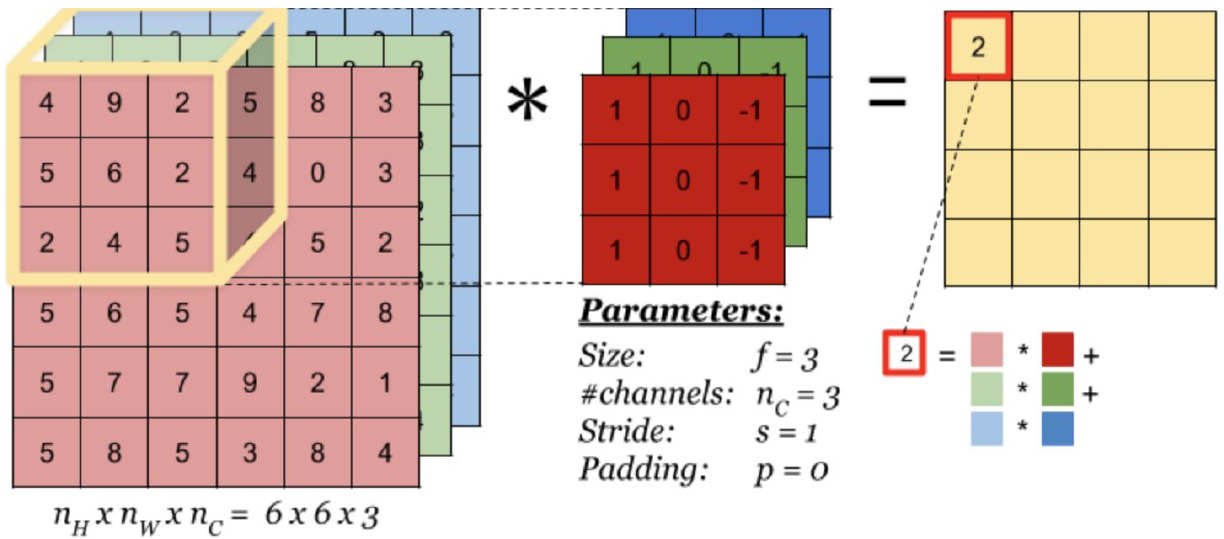
\includegraphics[width=0.45\textwidth]{Figures/kernel4.png}
    \vspace{-1\baselineskip}
    \begin{block}{Convoluted Operations}
        \begin{itemize}
            \item Filters correspond to the weights (or parameters)
            \item Hyperparameters
            \begin{itemize}
                \item Kernel Size
                \item Number of Filters
                \item Stride
                \item Padding
            \end{itemize}    
        \end{itemize}
    \end{block}
\end{frame}
\begin{frame}
    \frametitle{The Boilerplate}
    \centering
    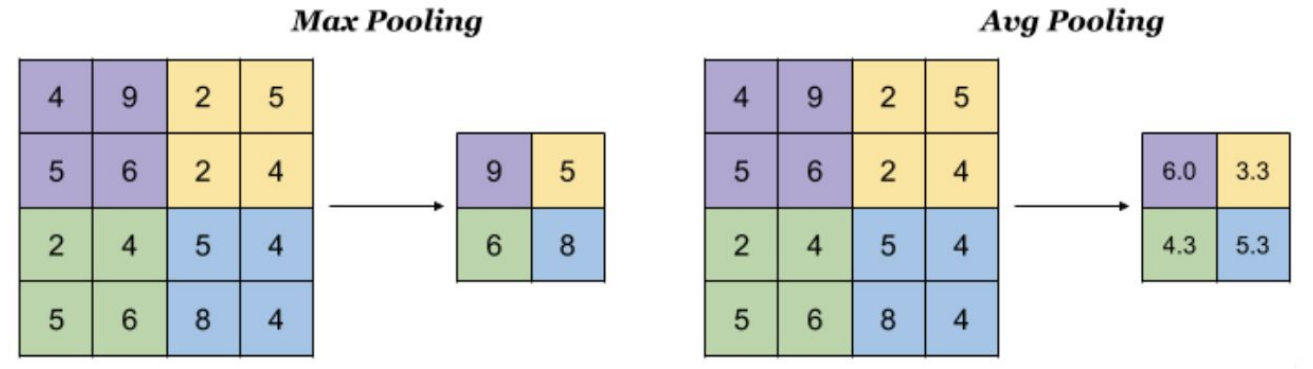
\includegraphics[width=0.7\textwidth]{Figures/pool.png}
    \begin{block}{pooling}
        \begin{itemize}
            \item Reduces size of representation
            \item reduces number of parameters
            \item provides translation invariance
            \item Controls overfitting        
        \end{itemize}
    \end{block}
\end{frame}
\begin{frame}
    \frametitle{The Boilerplate}
    \begin{block}{Regularization, Normalization}
        \begin{itemize}
            \item Dropout
            \item Batch Normalization       
        \end{itemize}
    \end{block}
\end{frame}


\section{Conclusion}
\subsection{Conclusion}
\begin{frame}
    \frametitle{Conclusion}
    \begin{block}{conclusion}
        \begin{itemize}
            \item Powerful
            \item Flexible
            \item Specific      
        \end{itemize}    
    \end{block}
\end{frame}
\subsection{Labs}
\begin{frame}
    \frametitle{Info About Labs}
    \begin{block}{Info About Labs}
        \begin{itemize}
            \item One lab - 4 parts
            \item Monday - done, Tuesday, Wednessday. 
            \item You will need the pods you used for the python lab
            \item you will find the adress in the studium page
        \end{itemize}    
    \end{block}
\end{frame}

\setbeamertemplate{background}{%
    \parbox[c][\paperheight]{\paperwidth}{%
        \vskip -8 ex \hskip -2 em
        
\includegraphics[height=1.5\paperheight]{Figures/gray.png}
    }  
      
}
\begin{frame}[plain]
    \vfill\hfill{\Huge\qquad\color{white} \zB Thank \zC you}\hfill\hfill\hfill\vfill
\end{frame}
\setbeamertemplate{background}{}

\end{document}
